\chapter{Planning in Four Subspaces}%
\label{chap:proposed_planning}
\textit{This chapter presents an existing motion planner~\cite{chen_fast_2018} that is extended to incorporate movable and unknown spaces next to the conventional free and obstacle spaces. The modification incentivizes the planner to find a path in free space but can pass through unknown or movable space as a last resort. The robot should first remove the blocking objects if a planned path crosses an unknown or movable subspace.\bs}

Finding a path between the start- and target configuration whilst avoiding collisions was presented in previous chapter. Now that path planner is modified; the modification extends the planner to incorporate movable and unknown space. The modified algorithm has four tuning parameters that can be tweaked; The \textit{step size} and \textit{search size} were discussed in previous chapter. The third and fourth tuning parameters are the fixed costs for crossing through movable or unknown space. These cost are added to the \textit{TotalPathCost}, which is redefined as:\bs

\[\mathit{Cost_{path}} = \mathit{MovableSpaceCost} + \mathit{UnknownSpaceCost} \sum_{i=1}^{n-1} \mathit{Distance}(\gls{c}_i, \gls{c}_{i+1})\]
\todo{In the pseudoce you talk about objectCost, here totalpathCost, unclear!}

The \textit{MovableSpaceCost} and \textit{UnknownSpaceCost} correspond to a fixed addition cost for a configuration in the path that crosses through movable or unknown subspace, respectively. Crossing through is defined as one or more nodes in the path lying in that subspace. If a path does not contain a node in movable space, \textit{MovableSpaceCost} will be 0, equivalent to unknown space and \textit{UnknownSpaceCost}. Optimizing the path for the lowest cost incentives the path planning algorithm to find a path around unknown or movable objects.\bs

The added fixed cost for a path crossing through a movable or unknown object motivates the path planner to find the shortest path around objects but prefers moving an object over making a large detour. Tuning the additional fixed cost for a path crossing through movable or unknown space balances the robot's decision between the length of a detour the robot is willing to drive, compared to pushing an object to free the path. Removing an unknown object bears more uncertainty than a movable object, motivating a higher cost to remove an unknown object compared to an known object. In the following pseudocode for the modified path planner is presented, changes compared to previously shown pseudocode are indicated in red.\bs

The proposed algorithm prevents planning a path through blocking objects except when no other option is available or a large detour can be prevented. No performance tests have been conducted on the modified path planner, apart from visual inspection. \Cref{fig:mp_push_or_drive} clearly shows the effect of varying \textit{UnknownSpaceCosts}.

\newpage
\todo{eleborate on the change compared to the previous existing algorithm}
\todo{Dubble check if only the parts in red are changed.}
\begin{algorithm}[H]
  \caption{Pseudocode for modified \ac{RRT*} path planning algorithm. Lines that contain changes compared to \Cref{pseudocode:proposed_rrt_star_all} are indicated with the red colour.}%
  \label{pseudocode:modified_proposed_rrt_star}
  \begin{algorithmic}[1]
    \State $\gls{nodesMP} \leftarrow x_{init}$
    \While{\textit{NotReachStop}}
        \State $\gls{nodeMP}_\mathit{rand} \leftarrow \mathit{Sample_{random}}$ \algorithmiccomment{Create, project and validate a new random sample}
      \State $\gls{nodeMP}_\mathit{nearest} \leftarrow \mathit{Nearest(\gls{nodeMP}_{rand}, \gls{nodesMP})}$
      \State $\gls{nodeMP}_\mathit{temp} \leftarrow \mathit{Project(\gls{nodeMP}_{rand}, \gls{nodeMP}_{nearest})}$
      \If{$\mathit{CollisionCheck(\gls{nodeMP}_{temp})}$}
      \State $\gls{nodeMP}_\mathit{new} = \gls{nodeMP}_\mathit{temp}$
      \State $\mathit{Cost_{toInitMin}} \leftarrow +\infty$ 
      \Else
      \State Continue
      \EndIf
      \State $X_\mathit{near} \leftarrow \mathit{NearestSet(\gls{nodeMP}_{new}, \gls{nodesMP})}$ \algorithmiccomment{Find and connect new node to parent node}
      \For{$\gls{nodeMP}_\mathit{near} \in X_\mathit{near}$}
    \State $\mathit{Cost_{temp}} \leftarrow \mathit{CostToInit}(\gls{nodeMP}_\mathit{near}) + \mathit{Distance}(\gls{nodeMP}_\mathit{near}, \gls{nodeMP}_\mathit{new}) + \textcolor{red}{\mathit{ObjectCost}(\gls{nodeMP}_\mathit{near}, \gls{nodeMP}_\mathit{new})}$
      \If{$\mathit{Cost_{temp}}  < \mathit{Cost_{toInitMin}}$}
      \State $\mathit{Cost_{toInitMin}} \leftarrow \mathit{Cost_{new}}$
      \State $\gls{nodeMP}_\mathit{minCost} \leftarrow \gls{nodeMP}_\mathit{near}$
      \EndIf
      \EndFor
      \If{$\mathit{Cost_{toInitMin}} == \infty$}
          \State Continue
      \Else
      \State $\gls{nodesMP}.add(\gls{nodeMP}_\mathit{new})$
      \State $E.\mathit{add}(\gls{nodeMP}_\mathit{minCost}, \gls{nodeMP}_\mathit{new})$
      \EndIf
      \State $\mathit{Cost_{pathMin}} \leftarrow +\infty$ 
      \For{$\gls{nodeMP}_\mathit{near} \in X_{near}$}\algorithmiccomment{\parbox[t]{.6\linewidth}{Check if the newly added node can lower cost for nearby nodes and if a both connectivity trees can be connected}}
      \If{$\mathit{InSameTree(\gls{nodeMP}_{near}, \gls{nodeMP}_{new})}$}
    \If{$\mathit{CostToInit(\gls{nodeMP}_{new})} + \mathit{Distance(\gls{nodeMP}_{new}, \gls{nodeMP}_{near})} +\textcolor{red}{\mathit{ObjectCost}(\gls{nodeMP}_\mathit{new}, \gls{nodeMP}_\mathit{near})} < \mathit{CostToInit(\gls{nodeMP}_{near})}$}
      \State $\mathit{E.rewire(\gls{nodeMP}_{near}, \gls{nodeMP}_{new})}$
      \EndIf
      \Else \algorithmiccomment{Add lowest cost path to the list of paths}

      \State $\mathit{Cost_{temp} \leftarrow CostToInit(\gls{nodeMP}_{new}) + Distance(\gls{nodeMP}_{new}, \gls{nodeMP}_{near})} + \mathit{CostToInit(\gls{nodeMP}_{near})}$
      % \State $\mathit{Cost_{temp} \leftarrow CostToInit(\gls{nodeMP}_{new}) + Distance(\gls{nodeMP}_{new}, \gls{nodeMP}_{near})} + \mathit{CostToInit(\gls{nodeMP}_{near}) + \textcolor{red}{ObjectCost(\gls{nodeMP}_{new}, \gls{nodeMP}_{near})}}$
      \If{$\mathit{Cost_{temp}  < Cost_{pathMin}}$}
      \State $\mathit{Cost_{pathMin}} \leftarrow \mathit{Cost_{temp}}$
      \State $\mathit{\gls{nodeMP}_{pathMin} \leftarrow \gls{nodeMP}_{near}}$
      \EndIf
      \EndIf
      \If{$Cost_{pathMin} == \infty$}
      \State Continue
      \Else
      \State $\mathit{P.addPath(\gls{nodeMP}_{new}, \gls{nodeMP}_{pathMin}, Cost_{pathMin})}$
      \EndIf
      \EndFor
    \EndWhile
  \end{algorithmic}
\end{algorithm}

\begin{figure}[H]
    \centering
    \begin{subfigure}{\textwidth}
    \centering
    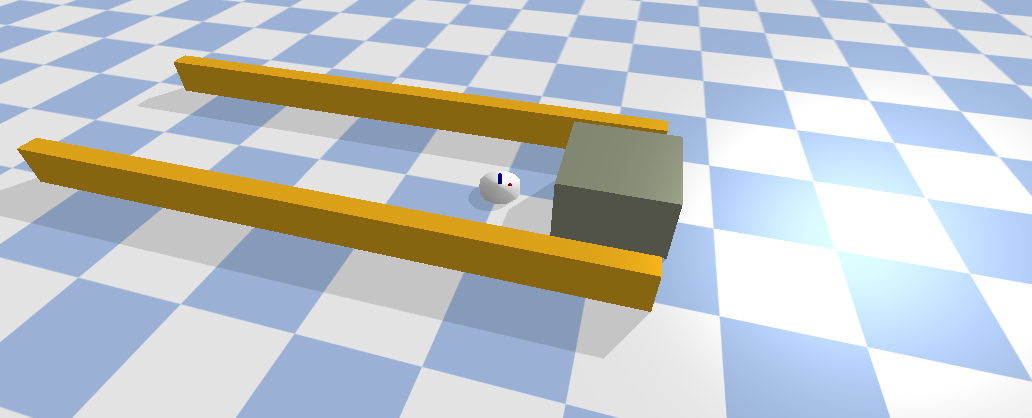
\includegraphics[width=0.8\textwidth]{figures/required_background/push_or_drive} \caption{Robot environment with the point robot, two yellow unmovable walls and an unknown brown box.\\The robot tasked to drive toward the opposite side of the brown box.}

\todo{Could you at least place a ghost pose on in this figure?}

    \end{subfigure}

    \begin{subfigure}{1.11\textwidth}
    \centering
    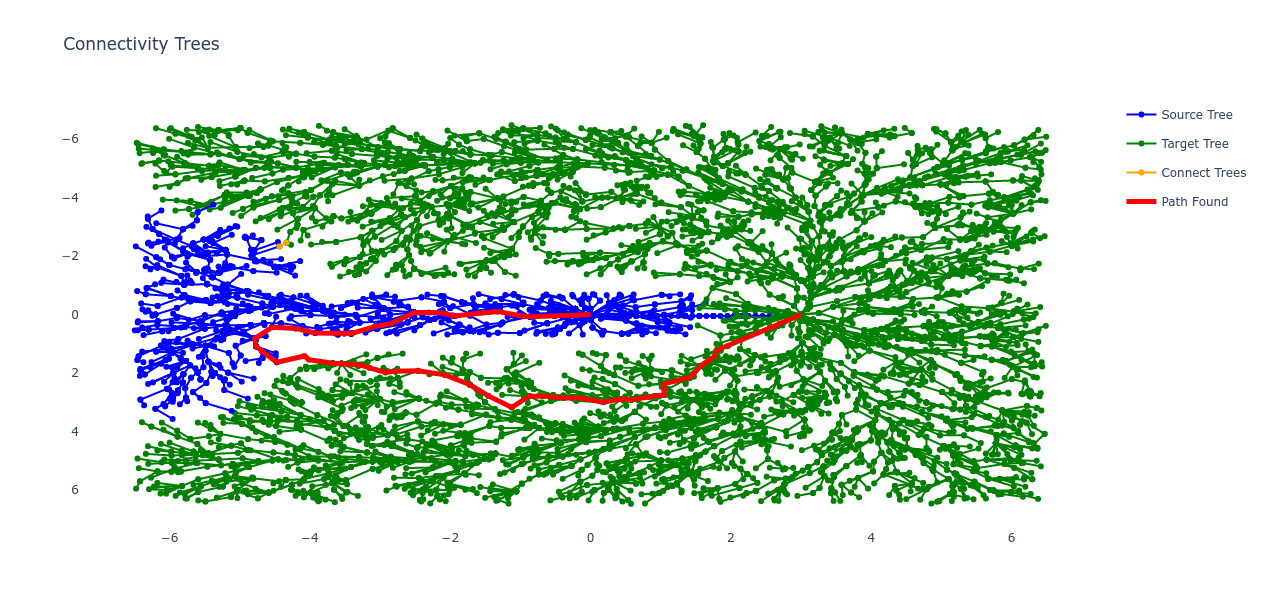
\includegraphics[width=\textwidth]{figures/required_background/mp/mp_high_fixed_cost}
    \caption{Visualization of the planned path around the brown box and yellow obstacles, with $\mathit{UnknownSpaceCost} = 1$.}
    \end{subfigure}

    \begin{subfigure}{1.11\textwidth}
    \centering
    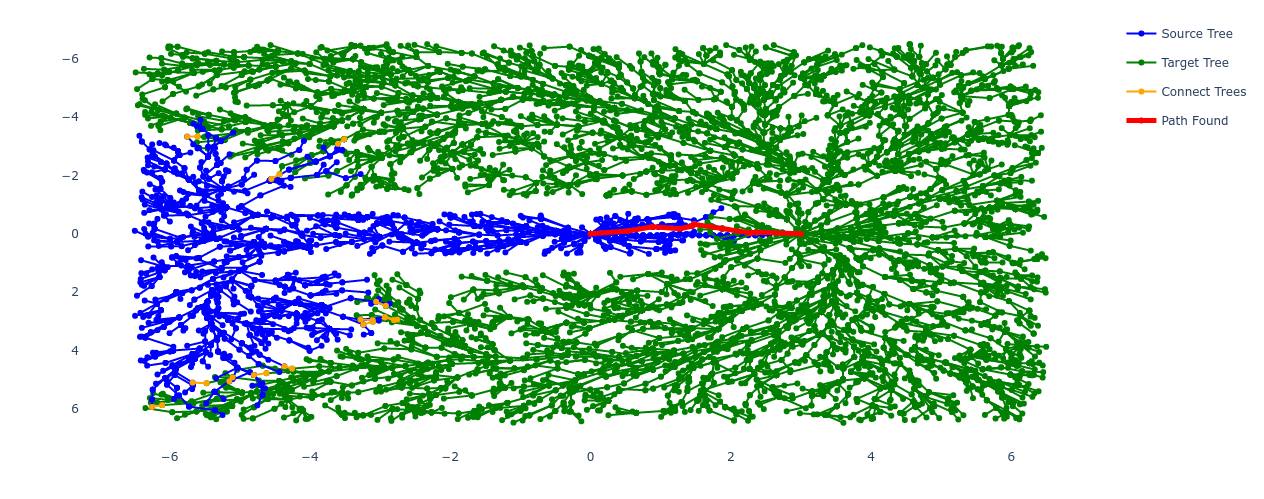
\includegraphics[width=\textwidth]{figures/required_background/mp/mp_low_fixed_cost}
    \caption{Visualization of the planned path going through the brown box, $\mathit{UnknownSpaceCost} = 0.5$.}
    \end{subfigure}
    \caption{Driving task and two path planned by the modified planning algorithm.}%
    \label{fig:mp_push_or_drive}
\end{figure}

Now that the modified path planner is discussed, the proposed robotic framework is discussed. The proposed framework relies on the required background from previous chapter, and relies on the modified path planner from this chapter.\bs



\todo{create a test that does things for the boxer robot, and it must have non-holonomic checker residing in the path}


% old manipulation section shit

% \subsection{Manipulation Planning}%
% \label{subsec:manipulation_planning}
% With a push, two objects are primarily involved, the pushed object and the robot. Generally, and in this thesis, the pushed object's configuration is more important than the robot's configuration. The robot is only a means to push the object toward the target configuration. At which final configuration the robot itself ends up is of lesser importance. As long as during the push, the robot does not collide with objects other than the pushed object, and constraints on the robot must be respected.\bs

% To plan a path that respects the constraints, \todo{Corrado: What does this mean? ->} the robot's configuration is generated for every newly added sample in the manipulation planning algorithm.

% \todo{Gijs For reachbailbpcheck, These lines just point out the name of the function again , there is no added information }
% The \textit{ReachabilityCheck()} (see \Cref{table:functions_for_proposed_rrt_star} and line 33 in \Cref{pseudocode:proposed_rrt_star}) generates the robot configuration to validate if a new sample is reachable from an existing sample. This additional configuration is stored to create only feasible paths that respect the applied constraints. When the stopping criteria are reached and the shortest path is found, the generated robot configurations are discarded. \Cref{fig:manipulation_plannig_local_planner} displays a visual example of the procedure.\bs

% \begin{figure}[H]
%     \centering
%     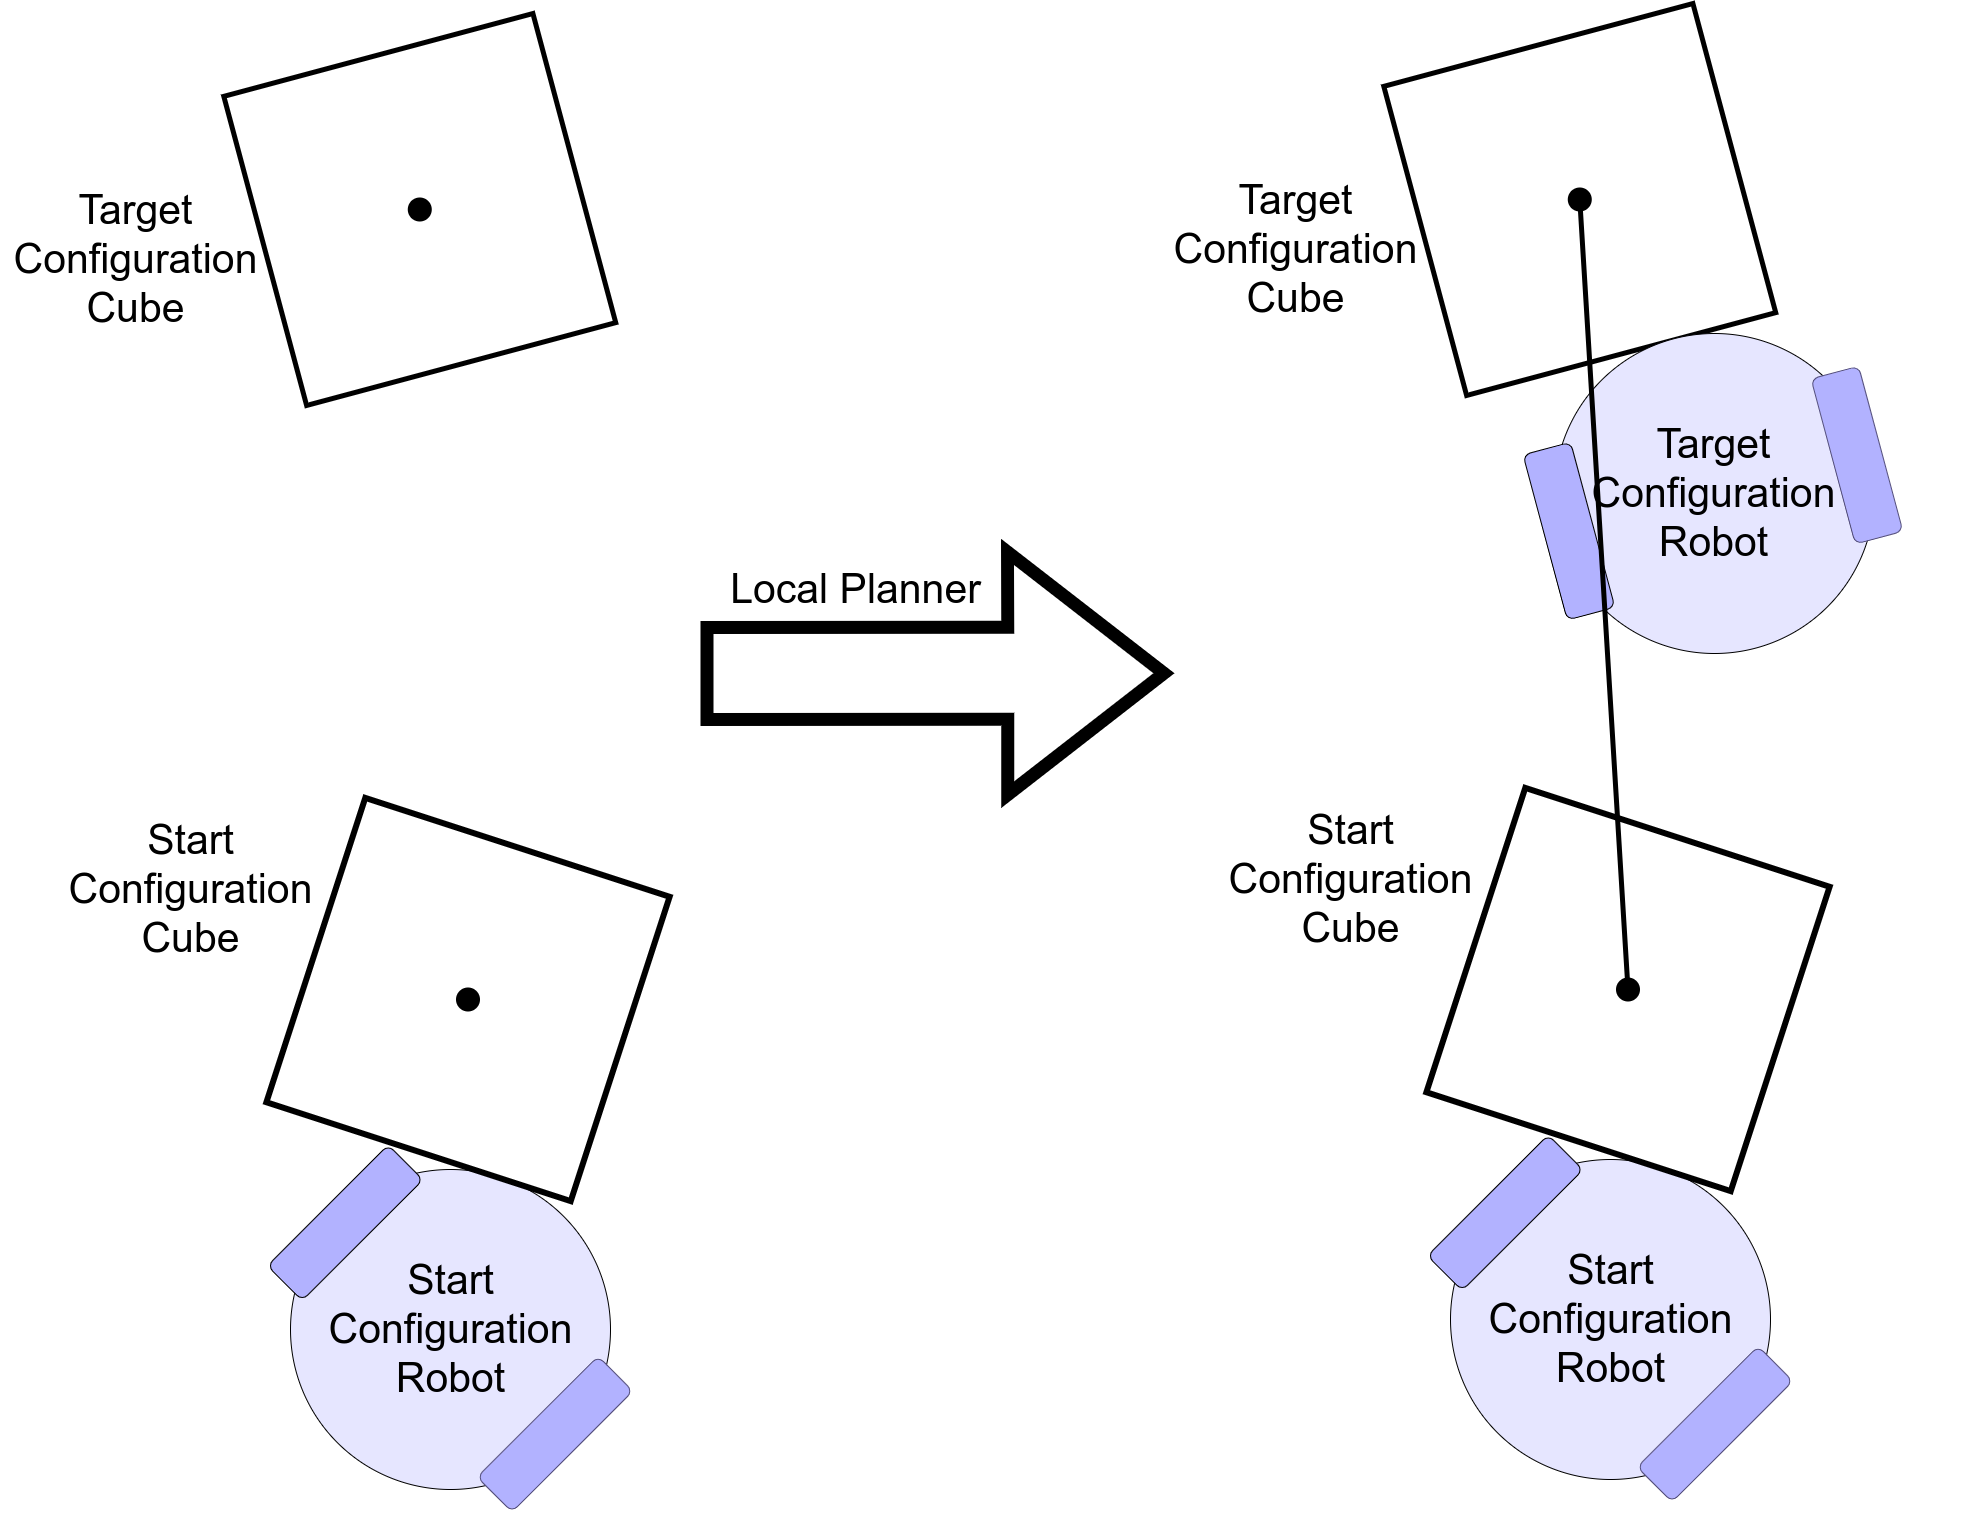
\includegraphics[width=0.6\textwidth]{figures/required_background/manipulation_local_planner}
%     \caption{Generating a new robot configuration whilst adding a sample to the connectivity tree during manipulation planning.}%
%     \label{fig:manipulation_plannig_local_planner}
% \end{figure}

 
\chapter{Proposed Robot Framework}%
\label{chap:h-graph_and_k-graph}
\textit{This chapter is dedicated to introducing and defining the proposed framework. The proposed framework consists of the \textbf{\acf{h-algorithm}}, the \textbf{\acf{h-graph}} and the \textbf{\acf{k-graph}}. The \ac{h-algorithm} acts on the \ac{h-graph} and is responsible for searching and executing action sequences to complete a specified task. \Cref{sec:h-graph} is dedicated to introducing and defining the \ac{h-graph}. Then the \ac{h-algorithm} is discussed and defined in \Cref{sec:h-algorithm}. The chapter finalizes with the \ac{k-graph} in \Cref{sec:k-graph}.\bs}

\section{Overview of the Proposed Framework}
\Cref{tikz:flowchart_proposed_method} presents a schematic overview of the interconnection of the \ac{k-graph}, \ac{h-algorithm} and the robot environment. The proposed framework could be augmented with a high-level planner that would transform a high-level task such as cleaning into the accepted format a list containing objects and corresponding target pose.\bs

\vspace{-0.4cm}
\begin{figure}[H] \centering
\begin{tikzpicture}[node distance = 1.5cm, auto]
    % Place nodes
    \node[draw=gray, rounded corners, inner sep=3ex, line width=7pt, fill=gray, fill opacity=0.4, minimum height=9.3cm, minimum width=5.8cm, yshift=2.50cm] (focusbox) {};
    \node[yshift=5.0cm, xshift=-1.5cm, align=left] at (focusbox) {\textbf{Thesis focus}};

   \node [outer sep=0cm] (environment) at (0,0)  {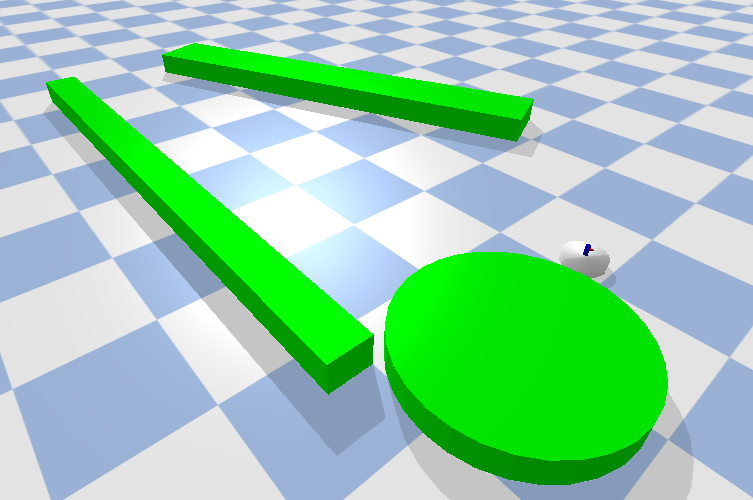
\includegraphics[width=4.6cm]{figures/proposed_method/example_environment.png}};

   \node [below, xshift=0.4cm, yshift=-.1cm, text width=5cm, align=left, outer sep=0cm] at (environment.north) {\textbf{Robot Environment}};

    \draw [myEvenLighterColor,
    rounded corners=0.3cm,
    line width=0.3cm]
    (environment.north west) --
    (environment.north east) --
    (environment.south east) --
    (environment.south west) -- cycle  ;

    \node [block,
    above of=environment,
    minimum height=1.5cm,
    minimum width=5cm,
    node distance=3.6cm,
    outer sep=0cm] (h-graph) {Hypothesis Algorithm};

    \node [block,
    above of=h-graph,
    node distance=2.5cm,
    minimum width=5cm,
    minimum height=1.5cm] (k-graph) {Knowledge Graph};

    \node [rectangle, draw,
    fill=myEvenLighterColor,
    text width=5em, text centered, rounded corners,
    right of=k-graph,
    minimum width=4cm,
    minimum height=1.5cm,
    node distance=7.5cm] (ontology) {Ontology};

    \node [rectangle, draw,
    fill=myEvenLighterColor,
    text width=5em, text centered, rounded corners,
    right of=h-graph,
    minimum width=4cm,
    minimum height=1.5cm,
    node distance=7.5cm] (planner) {High-level planner};

    % Draw edges
    \draw[-stealth] ([yshift=0.155cm, xshift=0.3 cm]environment.north) -- node [xshift=-.05cm, right] {\shortstack[]{sensor\\measurements}}([xshift=0.3 cm]h-graph.south) ;
    \draw[-stealth] ([xshift=-0.3 cm]h-graph.south) -- node [left] {robot input}([yshift=0.155cm, xshift=-0.3 cm]environment.north) ;
    \draw[-stealth] (planner.west) -- node [pos=0.37, above] {task}(h-graph.east);
    \draw[-stealth] ([xshift=-0.3cm]k-graph.south) -- node [left] {\shortstack[]{action\\suggestions}}([xshift= -0.3cm]h-graph.north) ;
    \draw[stealth-] ([xshift=0.3cm]k-graph.south) -- node [right] {\shortstack[]{action\\feedback}}([xshift= 0.3cm]h-graph.north) ;
    \draw[-stealth] (k-graph.east) -- node [xshift=-0.1cm, above, pos=0.63] {\shortstack[]{environment\\knowledge}}(ontology.west);
    \draw[stealth-] ([xshift=0.3cm]ontology.south) -- node [right] {\shortstack[]{query}}([xshift=0.3cm]planner.north);
    \draw[-stealth] ([xshift=-0.3cm]ontology.south) -- node [left] {\shortstack[]{output}}([xshift=-0.3cm]planner.north);
    \draw[stealth-] (planner.south) |- ++ (2,-1) node[near end, above] {\shortstack[]{High-level\\task}};
    \end{tikzpicture}
\caption{Flowchart representation of the proposed robot framework.}%
\label{tikz:flowchart_proposed_method}
\end{figure}

The block containing the \ac{h-algorithm} in \Cref{tikz:flowchart_proposed_method} orchestrates the generation and execution of action sequences. In doing so, it creates a \ac{h-graph}, first the \ac{h-graph} is introduced and discussed, then the \ac{h-algorithm} is introduced and discussed.\bs

\section{Hypothesis Graph}%
\label{sec:hgraph}
The \ac{halgorithm} is responsible for generating action sequences, called hypothesis. An hypothesis consists of a list of successive edges in the \ac{hgraph} from start to target node in the \ac{hgraph}. When all subtasks in a task are completed, the \acf{halgorithm} halts and concludes the task successfully completed. A search in the joint configuration space is avoided because an edge only operates in a single mode of dynamics, such as driving or pushing. When an object cannot directly be steered toward its target location new nodes are generated which need to be completed before the original object can be steered toward its target location. An example of when an object cannot directly be steered toward its target state is because the path is blocked by another object. A hypothesis, consisting of a list of edges that represent actions in the robot environment might succeed or fail. \Cref{tikz:flowchart_hgraph} displays a flowchart explaining how new nodes and edges are generated in the \ac{hgraph}. Successfully completed edges eventually result in completed subtasks, failed edges trigger replanning that will restart the search to a hypothesis.\bs

The \ac{halgorithm} with the \ac{hgraph} have a familiar structure compared to some recent literature~\cite{ellis_navigation_2022,wang_affordancebased_2020}. An important distinction is that the proposed method in this thesis aims to combine the 3 topics: learning object dynamics, solving \ac{NAMO} problems and nonprehensile pushing. Recent literature is able to only combine one or two topics of the three.\bs

In the upcoming section the \ac{hgraph} is defined and discussed in \cref{subsec:hgraph_definition}. The \ac{halgorithm} is then discussed and in \cref{subsec:halgorithm}, where an explanation is provided on how the \ac{halgorithm} searches for a solution in the joint configuration space. The section is concluded with an extensive example.\bs

\subsection{Definition}%
\label{subsec:hgraph_definition}%
Before defining the \ac{hgraph}, some definitions are defined on which the \ac{hgraph} depends. First, recall the \textbf{state} defined in the \cref{sec:problem_description}.\bs

An object holds the information about an object.\\Formally, a \textbf{object},  $obst_{id}(k) = \left\langle s(k), shape \right\rangle $\bs

where $shape$ is linked to a 3D representation of the object which is used to construct the configuration space.\bs

An object node represents an object in a state.\\Formally, a \textbf{objectNode}, $V^{obst}_{id} =\left\langle \textrm{status}, obst(k)\right\rangle $\\where status indicates if the node has been visited in the \ac{hgraph}. $\textrm{status} = (Initialised, Completed, Failed)$\bs

An edge describes the details of how a node transitions to another node in the \ac{hgraph}. In the robot environment, an edge represents a change of state for an object. System identification and performing an action such as pushing or driving both change the state of objects in the robot environment, but because are very different, the edges are split into 2 categories. IdentificationEdges that collect system \ac{IO} data and convert that into a system model. And actionEdges that plan and track a motion from a start to a target state. Formally:\bs

A \textbf{identificationEdge},
\todo[inline]{define identificationEdge, currently hard coded models are used in the implementation}

A \textbf{actionEdge}, $\tau_{(from, to)} = \left\langle \textrm{status}, id_{from}, id_{to}, \textrm{verb}, \textrm{controller},\textrm{dynamic model}, \textrm{path}\right\rangle$\bs

with $id_{from}$ and $id_{to}$ indicating the node id of the node in the \ac{hgraph} where the edge start from and point to respectively, $verb$ an English verb describing the action the edge represents, the controller contains the controller used for driving the robot, the dynamic model is the dynamic model used by the controller, path a list of configurations indicating the path connecting a start- to target node.\bs
\todo[inline]{Martijn: what does this mean: "the controller contains the controller..."?}

A $verb = \{\textrm{driving, pushing}\}$.\bs

Now the nodes and edges have been defined, the \ac{hgraph} can be defined.\bs

Formally, a \textbf{hypothesis graph}, $G^{hypothesis} = \left\langle V, E \right\rangle $ 
\\comprising $V = \{V^{ob}_{i}\}$, \quad $E \in \{\tau_{(i,j)}| V_i, V_j \in \{V^{ob} \}, i \neq j\}$.\bs

Most \ac{hgraph} components have now been defined. The status of an identification edge or action edge still remains undefined and requires some further explanation.\bs

\paragraph{Status, Types and Lifetime of edges}
Because system identification and tracking a path are so very different, the edges are split into two categories, identification edges and action edges. An identification edge, which is responsible for sending an input sequence to the system and recording the system output. That input/output sequence and assumptions on the system are the basis for system identification, techniques on various system identification methods are discussed in \cref{sec:sys_iden}. The goal is to create a dynamical model which is augmented with a corresponding controller is closed-loop stable.\bs

An identificationEdge, the status can be visualised in \cref{tikz:status_identification_edge}.\bs

\begin{figure}[H]
\centering
\begin{tikzpicture}[node distance = 2cm, auto, initial]
    \node [state, fill=my_dark_blue] (init_test_num) {IT\#t};
    \node [state, fill=my_light_blue, below of=init_test_num] (completed_test_num) {CT\#t};
    \node [state, accepting, fill=my_green, below of=completed_test_num] (completed) {CO};
    \node [state, accepting, fill=my_red, right of=completed_test_num, node distance=6cm] (failed) {FAIL};

 % arrows
    \draw [-stealth] ([xshift=-2cm]init_test_num.west) to node[near start,above]{\shortstack[]{select compatible\\sys. iden. method}} (init_test_num.west);
    \draw[-stealth] (init_test_num) edge[bend right] node[left]{Collect \ac{IO} data} (completed_test_num)
(completed_test_num) edge node[left]{create system model} (completed);
    \draw [-stealth] (completed_test_num) edge[bend right] node[right]{goto next start state} (init_test_num);
    \draw [-stealth] (completed_test_num) to node[]{Unable to reach next start state}  (failed.west);
    \draw [-stealth] (init_test_num) [out=0, in=90] to node[above]{Unable to reach next pos}  (failed.north);

\end{tikzpicture}
\caption{\acs{FSM} displaying the status of an identification edge}%
\label{tikz:status_identification_edge}
\end{figure}

\todo[inline]{some explainer on this status of iden edge}

The second type of edge is an actionEdge, containing a drive or push action. An actionEdge ready for execution contains all the necessary information to send input to the robot resulting in an object being steered toward it's target state. Before an edge is ready for execution it should be initialised properly, more specifically: initialised, path estimated should be performed, a system model must be initiated and path planning must be performed. Then finally the edge is ready to be executed and send input toward the robot, an \ac{FSM} of the actionEdge's status can be visualised in \cref{tikz:status_action_edge}.\bs

\begin{figure}[H]
\centering
\begin{tikzpicture}[node distance = 2cm, auto, initial]
    % \node [state, fill=lavenderIndigo] (init) {IN};
    \node [state, fill=my_purple] (init) {IN};
    \node [state, fill=my_dark_blue, below of=init] (path_exist) {PE};
    \node [state, fill=my_light_blue, below of=path_exist] (system_model) {SM};
    \node [state, fill=my_green, below of=system_model] (path_planned) {PP};
    \node [state, fill=my_yellow, below of=path_planned] (executing) {EX};
    \node [state, accepting, fill=my_orange, below of=executing] (completed) {CO};
    \node [state, accepting, fill=my_red] (failed) at ([xshift=4cm]$(system_model)!0.5!(path_planned)$) {FAIL};
    
 % arrows
    \draw [-stealth] ([xshift=-2cm]init.west) to node[near start,above]{select controller} (init.west);
    \draw[-stealth] (init) edge node[left]{graph-based path estimation} (path_exist)
      (path_exist) edge[bend right] node[left]{load in system model} (system_model)
(system_model) edge[bend right] node[left]{motion planning} (path_planned)
(path_planned) edge[bend right] node[left]{goto execution loop} (executing)
(executing) edge[bend right] node[left]{completed} (completed);

    \draw [-stealth] (init.east) [out=0, in=90] to node[xshift=0.1cm, right]{path non-existence proven}  ([yshift=-0.03cm,xshift=0.2cm]failed.north);
    \draw [-stealth] (path_exist.east) [out=0, in=90] to node[xshift=-0.6cm,yshift=0.55cm, above]{\shortstack[l]{system\\identification\\error}}  ([yshift=-0.03cm,xshift=-0.2cm]failed.north);
    \draw [-stealth] (system_model.east) [out=0, in=180] to node[xshift=0.1cm, yshift=0.3cm, above]{\shortstack[l]{motion\\planning\\error}} (failed.west);
    node[right]{motion planning error}  
    ([yshift=-0.3cm]failed.west);
    \draw [-stealth] (executing.east) [out=0, in=-90] to node[xshift=0.1cm,right]{fault detected}(failed.south);

\end{tikzpicture}
\caption{\acs{FSM} displaying the state of an action edge}%
\label{tikz:status_action_edge}
\end{figure}

% \par\smallskip\noindent
\centerline{\begin{minipage}{0.8\textwidth}
\begin{enumerate}
  \item[INITIALISED (IN)] The edge is created with a source and target node which are present in the \ac{hgraph}. A choice of controller is made.
    \item[PATH EXISTS (PE)] A graph-based search is performed to validate if the target state is reachable assuming that the system is holonomic.
    \item[SYSTEM MODEL (SM)] A dynamics system model is provided to the controller residing in the edge.
    \item[PATH PLANNED (PP)] Resulting from a sample-based planner, a path from start to target state is provided. 
    \item[EXECUTING (EX)] The edge is currently receiving observations from the robot environment and sends back robot input. 
    \item[COMPLETED (COMPL)] The edge has driven the system toward its target state and its performance has been calculated.
    \item[FAILED (FAIL)] An error occurred, yielding the edge unusable. 
\end{enumerate}
\end{minipage}}
\par\smallskip

\Cref{tikz:status_action_edge} shows that many steps must successfully be completed before the robot can start executing. The performance of an edge during execution, measured in various metrics (\cref{sec:proposed_method_metrics} is dedicated to metrics) is dependent on many aspects. Such as the choice of controller, the path estimation, the system model yielded by the identification edge and the path yielded by motion planning. Now that he \ac{hgraph} is defined, let's see how it is generated in the upcoming section.\bs

\subsection{\acl{halgorithm}}%
\label{subsec:halgorithm}
This section will provide a mathematical description of the proposed \ac{halgorithm}, the search and execution loop are discussed. The section will finalise with 4 examples. First, let's look into the math of the \ac{halgorithm}.\bs

\todo[inline]{a mathematically solid describtion of your backward search algorithm}

During a backward search, edges are added pointing toward the target node (or to nodes that point toward the target node). Trying to connect the robot node through a list of succesive directed edges to a target node. If such a path has been found in the \ac{hgraph}, a hypothesis has been found and the robot can start executing edges.

A flowchart of the \ac{halgorithm} is presented in \cref{tikz:flowchart_hgraph}. Compared to the mathematical description of the \ac{halgorithm} the flowchart provides more detail, including an eleborate description for every block in the flowchart (see \cref{table:explainer_hgraph_figures_nodes}). The flowchart includes path estimation, planning and the behavior when failure occures. A connection point to the \ac{kgraph} and robot environment are included. The blocks in the flowchart indicate which action they take and where, such as the configuration space, the \ac{kgraph} or the \ac{hgraph}. With the flowchart is straigtforward to see how the \ac{halgorithm} connects to the status of edges, with the mathematical description of the \ac{halgorithm} that is harder so see. Compared to the flowchart the mathematical description is a abstacted version, leaving many details out that are related to the robot in this thesis. An abstracted mathematical description is simpler and encompasses a broader field of robots. So could the mathematical description also be applied to another robot such as a movable robot with robot arm and gripper. The flowchart encompasses to many details to be applied after such an change in robot hardware. 

% \newgeometry{left=1.1cm,bottom=0.1cm,top=1.9cm,headsep=0.1in,heightrounded}

\newpage
\vspace*{-1.2cm}
\hspace{-1.2cm}
\begin{minipage}{10cm}
\begin{figure}[H] 
\centering
\begin{tikzpicture}]
  [node distance = 3cm] 

    % Nodes
    \node [block, fill=yellow!50, line width=2pt, dashed] (first) {Create Start and Target Nodes};
    
    % legend
    \node[text width=2.8cm, yshift=0.6cm, right of=first, node distance=7cm, text centered, rounded corners, minimum height=1em, label={[name=lab, yshift=0.4cm, left]\textbf{Legend}}] (legend1) {\small Update KGraph};
    \node[rectangle, draw, left of=legend1, fill=green!50, rounded corners, minimum height=1em, minimum width=1cm, node distance=2cm] (legend1color) {};
    
    \node[text width=2.8cm, below of=legend1, text centered, minimum height=1em, node distance=0.7cm] (legend2) {\small Query KGraph};
    \node[rectangle, draw, left of=legend2, fill=red!40, rounded corners, minimum height=1em, minimum width=1cm, node distance=2cm] (legend2color) {};
   
    \node[text width=2.8cm, below of=legend2, text centered, minimum height=1em, node distance=0.7cm] (legend3) {\small Update C-Space};
\node[rectangle, draw, left of=legend3, fill=yellow!50, rounded corners, minimum height=1em, minimum width=1cm, node distance=2cm] (legend3color) {};
    
    \node[text width=2.8cm, below of=legend3, text centered, minimum height=1em, node distance=0.7cm] (legend4) {\small action in HGraph};
    \node[rectangle, draw, left of=legend4, rounded corners, minimum height=1em, minimum width=1cm, node distance=2cm, line width=2pt, dashed] (legend4color) {};
 
    \node[text width=2.8cm, below of=legend4, text centered, minimum height=1em, node distance=0.7cm] (legend5) {\small action in C-Space};
\node[rectangle, draw, left of=legend5, rounded corners, minimum height=1em, minimum width=1cm, node distance=2cm, line width=2pt] (legend5color) {};

    % nodes, Path exists 
    \node [decision, below of=first, node distance=2.6cm, line width=2pt] (path_existence) {Estimate Path Existence};
    \node [decision, left of=path_existence, node distance=4.5cm, line width=2pt, dashed] (subtasks) {Is There an Unfinished Subtask};

    \node [block, above of=subtasks, node distance=2.8cm] (no_solution_found) {Task Finished};
    
    % nodes, Knowledge available
    \node [decision, fill=red!40, below of=path_existence, node distance=3.2cm, inner sep=0.5mm] (know_avail) { Knowledge Available };
    \node [decision, fill=red!40, right of=know_avail, node distance=3.5cm, inner sep=0.5mm] (know_good) {Knowledge Usable};
    \node [decision, right of=know_good, node distance=3.5cm, text width=1.7cm] (movable) {\vspace{0.1cm}\shortstack[]{Object\\Movable or\\Unknown}};
    \node [block, left of=know_avail, node distance=3cm, line width=2pt, dashed] (impossible) {Impossible Node};
    
    % nodes, Generate new edge
    \node [decision, below of=know_avail, node distance=3.2cm, line width=2pt, inner sep=0.5mm, dashed] (goto_sys_iden) {Generate Random Action};

    \node[block, right of=goto_sys_iden, node distance=3.5cm, line width=2pt, dashed] (no_trans_found) {All Possible Actions Failed};
    
    
    % Motion/Manipulation planning 
    \node [decision, below of=goto_sys_iden, node distance=3.5cm] (single_multi) {Action Type};

    \node [decision, line width=2pt, dashed, left of=single_multi, node distance=3.7cm] (model_avail_single) {Model Available};
    \node [decision, line width=2pt, dashed, right of=single_multi, node distance=3.7cm] (model_avail_multi) {Model Available};
    \node [block, line width=2pt, dashed, left of=model_avail_single, node distance=2.8cm] (sys_iden_single) {Add Drive Sys. Iden. Node};
    \node [block, line width=2pt, dashed, right of=model_avail_multi, node distance=2.8cm] (sys_iden_multi) {Add Push Sys. Iden. Node};
    \node [block, line width=2pt, dashed, below of=single_multi, node distance=2.7cm] (move_object) {Add Node to Move Object};
    \node [block, line width=2pt, left of=move_object, node distance=3.7cm] (motion_planning) {Motion Planning};
    \node [block, line width=2pt, right of=move_object, node distance=3.7cm, text width=2.1cm] (manipulation_planning) {Manipulation Planning};

    \node [decision, line width=2pt, dashed, minimum width=2.3cm, below of=move_object, node distance=2.3cm, xshift=1.75cm] (drive_to_push_position) {Robot Close to Push Pose};
    \node [block, line width=2pt, dashed, minimum width=2.3cm, below of=move_object, node distance=2.3cm, xshift=-1.75cm] (goto_push_position) {Add Node to Drive to Push Pose};
  
    \node [decision, line width=2pt, above of=sys_iden_single, node distance=3.5cm] (add_drive_node) {Robot Close to Object};

    \node [block, dashed, line width=2pt, above of=add_drive_node, node distance=3.2cm] (do_add_drive_node) {Add Node to Drive to Object};

    % nodes, Path to target
    \node [decision, below of=motion_planning, node distance=4.0cm, line width=2pt, dashed] (global_path) {Path to Target}; 
1   \node [decision, right of=global_path, node distance=7.4cm, line width=2pt, dashed] (first_action) {First Action Planned};

    \node [decision, right of=first_action, diagonal fill={yellow!50}{green!50}, node distance=3cm] (execute) {Execute};
     
    % nodes, Target node reached 
    \node [decision, below of=global_path, node distance=3cm, line width=2pt, dashed] (target_node_reached) {Target Node Reached};
    \node [block, left of=target_node_reached, node distance=3cm] (end) {Subtask Successfully Completed};
    
    % Edges
    \path[line] ++(0,1.2) -- node[yshift=0.2cm, above]{task} (first);
    \path[line] (first) -- node[midway](to_path_exists){}(path_existence); 
    
    % edges, Path exists 
    \path[line] ([xshift=0.2cm, yshift=-0.2cm] path_existence.south west) -| node[near start, xshift=-0.4cm, above] {no path found} (impossible.north);
    \path[line] (subtasks.north) --  node[left] {no} (no_solution_found);
    \path[line] (path_existence) -- node[xshift=0cm, yshift=0.15cm, left] {path found} (know_avail); 
    \path[line] (subtasks.east) -- node[above] {yes} (path_existence.west);
    
    % edges, Knowledge available
    \path[line] (know_avail) -- node[above] {yes} (know_good); 
    \path[line] (know_good) -- node[yshift=0.1cm, above] {no} (goto_sys_iden); 
    \path[line] (know_avail) -- node[left](toward_new_trans) {no} (goto_sys_iden); 
    \draw[-stealth] (know_good.east) -- node[above] {yes} (movable.west);
    
    % \draw[-]  ([xshift=3.2mm]toward_new_trans.center) -| node[near start, above] {no} (know_good.south);
    \draw[-](impossible.west) -- +(-0.47,0); 
     
    \draw[-]  ([xshift=2.75cm, yshift=6.6cm]know_avail.center) --  node[at start, above] {\shortstack[]{action\\suggestions}} ([xshift=1.75cm, yshift=3.75cm]know_avail.center) -- ([xshift=1.75cm, yshift=3.75cm]know_avail.center);

    \draw[-stealth]  ([xshift=1.75cm, yshift=3.75cm]know_avail.center) --  ([xshift=1.75cm, yshift=1.75cm]know_avail.center) -- (know_avail.north east);
    \draw[-stealth]  ([xshift=1.75cm, yshift=1.75cm]know_avail.center) -- (know_good.north west);
    \draw [draw=white,double distance=\pgflinewidth,ultra thick] (path_existence.east) -- +(2cm,0);
    
    % edges, Generate new edge
    \draw[-] (move_object.south) |- +(-7.70,-0.3);
    \draw [draw=white,double=black,double distance=\pgflinewidth,ultra thick] (motion_planning.south) -- +(0,-1cm);
    \draw[-stealth] (motion_planning.south)  -- ([yshift=-1cm]motion_planning.south) -| node[near start, left] {success} (global_path.north);
    \draw[-stealth] (manipulation_planning.south) |- node[near start, right] {success} (drive_to_push_position.east);
    \draw[-] ([xshift=0.1cm,yshift=0.1cm] drive_to_push_position.north west) -- node[at start, xshift=-0.5cm, above] {yes} ++(-4.75cm,0);
    \draw[-stealth] (drive_to_push_position.west) |- node[xshift=-0.3cm, above] {no} (goto_push_position.east);
    \draw[-] (goto_push_position.west) -- ++(-0.77cm, 0); 

    \draw[-] (motion_planning.west) -- node[above] {failure} +(-2.98,0);
    \draw[-] (manipulation_planning.east) -| node[near start, above] {failure} ([xshift=4.7cm,yshift=-0.6cm]no_trans_found.south) -- ([yshift=-0.6cm]no_trans_found.south);
    
    % edges, Single/Multi body
    \draw[-stealth] (single_multi.west) -- node[above] {driving} (model_avail_single);
    \draw[-stealth] (single_multi.east) -- node[above] {pushing} (model_avail_multi);
    \draw[-stealth] (model_avail_single.south) -- node[left] {yes} (motion_planning.north);
    \draw[-stealth] (model_avail_single.west) -- node[above] {no} (sys_iden_single);

    \draw[-stealth] (model_avail_multi.east) -- node[above] {no} (sys_iden_multi);
    \draw[-stealth] (motion_planning.east) -- node[above] {blockade} (move_object);
    \draw[-stealth] (manipulation_planning.west) -- node[above] {blockade} (move_object);
    \draw[-stealth] (goto_sys_iden) -- node[above] {fail} (no_trans_found);
    \draw[-] (sys_iden_single.north) --  ([yshift=0.56cm]sys_iden_single.north);
    \draw[-] (sys_iden_multi.north) |-  ([yshift=-0.6cm]no_trans_found.south);
    \draw[-] (no_trans_found.south) -- ++(0,-0.6cm) --([xshift=-8cm, yshift=-0.6cm]no_trans_found.south);
    \draw [draw=white,double=black,double distance=\pgflinewidth,ultra thick] (goto_sys_iden.south) -- node[yshift=0.1cm, right] {success}(single_multi.north);
    \draw[-stealth] ([yshift=0.05cm] goto_sys_iden.south) -- (single_multi.north);
    
    \draw[-] (movable.south) |- node[near start, left] {\shortstack[r]{yes, generate\\suggested\\edge}} ([xshift=-1.5cm, yshift=-1.4cm]movable.south) |- ([yshift=0.3cm]single_multi.north);
    \draw [draw=white,double distance=\pgflinewidth,ultra thick]  ([xshift=-1cm]movable.north) -- ([xshift=-7.2cm]movable.north);

    \draw[-] (movable.north) -- node[xshift=3cm, above]{no, object is obstacle}([xshift=-10cm]movable.north);
    % HERE
    \draw [draw=white,double=black,double distance=\pgflinewidth,ultra thick] ([xshift=5.5cm,yshift=0.3cm]single_multi.north) -- ([xshift=5.5cm, yshift=2cm]single_multi.north);
    % \draw[-] (know_good.east) -| node[above]{yes} ([xshift=5.5cm, yshift=0.2cm]single_multi.north) -- ([yshift=0.2cm]single_multi.north);

    
    \draw[-stealth] (add_drive_node.north) -- node[left] {no} (do_add_drive_node.south);
    \draw[-] (add_drive_node.north east) -- node[left] {yes} ++(1.3cm,1.3cm);
    \draw[-] (do_add_drive_node.east) --  ++(1.10cm,0);
    % edges, Path to target
    \path[line] (global_path) -- node[above] {yes} (first_action);
    \path[line] (first_action.east) -- node[above] {yes} (execute);
    \path[line] (global_path.west) -| node[xshift=1cm, left, above, near start] {no}  ([xshift=-2.8cm, yshift=8cm]global_path.west) -|  (subtasks.south); 
   
    \draw[-stealth] (first_action.north east) -- node[near end, left] {no} ([xshift=1.7cm, yshift=0.39cm]first_action.north) |- ([yshift=-0.35cm]single_multi.south) -- (single_multi.south);
    \draw [draw=white,double=black,double distance=\pgflinewidth,ultra thick] (manipulation_planning.east) -- +(1cm,0);
    \draw [draw=white,double=black,double distance=\pgflinewidth,ultra thick] (manipulation_planning.north) -- +(0,0.6cm);
    \draw [draw=white,double=black,double distance=\pgflinewidth,ultra thick] (single_multi.north west) -- ([xshift=1cm,yshift=-0.425cm] add_drive_node.south east);
    \draw[-stealth] (single_multi.north west) -- node[xshift=-0.7cm, yshift=0.4cm, near start, above, right] {identification} (add_drive_node.south east);

    \draw[-stealth] (model_avail_multi.south) -- node[near start, left] {yes} (manipulation_planning.north);
    
    \draw[-stealth] ([yshift=0.2cm, xshift=0.2cm]execute.south east) --  ([yshift=-0.8cm, xshift=1.2cm]execute.south east) -- node[at end, left] {robot input, action feedback} +(0,-2.7cm);
    
    \draw[stealth-] ([yshift=-0.2cm, xshift=-0.2cm]execute.south east) --  ([yshift=-1.2cm, xshift=0.8cm]execute.south east) -- node[left, at end] {sensor measurements} +(0, -1.8cm);
    
    \path[line] (execute.south) |- node[near start, left] {success} (target_node_reached.east);
    \draw[-stealth] (execute.east) -- node[above] {failure} ([xshift=1.5cm]execute.east) |- (path_existence.east);
    \draw[-] (end.north) -- ++(0,2.07cm);
    
    
    % edges, Target node reached 
    \path[line] (target_node_reached.north) -- node[left] {no} (global_path.south);
    \path[line] (target_node_reached.west) -- node[above] {yes} (end.east);

\end{tikzpicture}
% \vspace{-5cm}
\caption{Flowchart displaying the hypothesis graph's workflow.}%
\label{tikz:flowchart_hgraph}% 
\end{figure}

\end{minipage}
\newpage


\begin{table}[H]
\centering
\rowcolors{2}{white}{myLightColor}
\begin{tabular}[t]{>{\raggedright}p{3.5cm}>{\raggedright\arraybackslash}p{10.5cm}}
  \textbf{Node name} & \textbf{Description of actions taken}\\\toprule
  Task Finished & log all metrics for the \ac{hgraph}, then deconstruct \ac{hgraph}.\\
  Create Start and\newline Target Nodes & Generate a robot node and the start and target nodes for every subtask in the task.\\
Update Current Subtask & Select an unfinished subtask or update current subtask. Use the backward search technique. The \textit{current\_start\_node} and \textit{current\_target\_node} are updated. When all subtask have been addressed, conclude task is finished. \\
Estimate Path\newline Existence & Check if a path exists between \textit{current\_start\_node} and \textit{current\_target\_node} whilst assuming that the object is holonomic.\\
Add Node to\newline Drive to Object & Add a node before the \textit{current\_target\_node}.\\
Unfeasible Node & Update node's status to unfeasible because is can not be completed, log failed Edge.\\
Knowledge Available& Query the \ac{kgraph} for action suggestion to connect \textit{current\_target\_node} to \textit{current\_target\_node}\\
Knowledge Usable& Check if a suggested action is not on the blacklist.\\
Object Movable & Check if object is classified as movable\\
Robot Close to Object& Check if the object is inside directly reachable free space of the robot \\
Generate Random\newline Action& Randomly sample a controller with a compatible system identification method that is not on the blacklist. \\
All Possible Actions Failed & Every possible action is on the blacklist for the \textit{current\_target\_node}, update \textit{current\_target\_node} status to failed.\\
Add Drive System Identification Edge & Adds identification edge between a newly generated node and the drive action edge source node. \\
Model Available& Checks if the drive action edge contains a system model. \\
Action Type& Checks the action type. \\
Model Available& Checkif the push action edge containts a system model. \\
Add Push System\newline Identification Edge& Adds identification edge compatible with push action edge. \\
Motion Planning& Search a path for the \textit{current\_edge}, detect blocking objects. \\
Add Node to Free Path & Search closeby pose for object to free path. Create node to push object toward that pose. \\
Manipulation Planning & Search a path for the \textit{current\_edge}, detect blocking objects.\\
Add Node to Drive\newline to Push Pose& Create node to drive toward push pose, add before action edge. \\
Robot Close to\newline Push Pose & Check if the robot is overlapping with the best push position. \\
Path to Target& Is there a path from robot to target node in the \ac{hgraph}, then set first edge to \textit{current\_edge} otherwise update subtask.\\
First Action Planned&  Check if motion/manipulation planning was performed. \\
Execute& Execute the \textit{current\_edge}, update \ac{hgraph} after completion, log failed hypothesis if a fault is detected. \\
Subtask Succesfully\newline Completed& Log hypothesis metrics. \\
Target Node Reached& Check if the target node is reached.\\
\end{tabular}
\caption{Eleborate information on actions taken by blocks in \cref{tikz:flowchart_hgraph}.}%
\label{table:explainer_hgraph_figures_nodes}
\end{table}

When all tuning parameters are set, the \ac{hgraph} is initialized and a task is provided, there is only a single access point toward the \ac{hgraph}. A function \textit{respond(observation)} that provides the \ac{halgorithm} with sensor measurements of the environment with the argument \textit{observation}. The function \textit{respond($\cdot$)} returns control in put for the robot. In this theses, the sensor measurements are the configuration of objects in the environment. Recall that the perfect-sensor assumption, assumption~\ref{assumption:perfect_object_sensor} that makes access to the exact configuration of every object possible.\bs


\paragraph{The Blacklist}%
Undesirable behavior is to generate an edge that fails, only to regenerate and fail again. This infinite behavior is prevented by the blacklist. When the \ac{halgorithm} connects two nodes with an action edge, the possible parameterizations (controller and system model) are filtered. Thus any parameterisation that is on the blacklist for this specific node (to which the action edge would point toward) cannot be created again for the lifetime of the \ac{hgraph}. An example where the blacklist can be seen in action is \cref{fig:failure_in_hgraph}.\bs

\todo[inline]{math def for blacklist on the nodes}


\subsection{The Search and the Execution loop}%
\label{subsec:two_loops}
In \cref{tikz:flowchart_hgraph} two main loops can be identified, see \Cref{fig:two_loops_identified}. These loops are the search loop, and the execution loop.\bs

\begin{figure}[H]
    \centering
    \includegraphics[width=7cm]{figures/two_loops_identified}
    \caption{The search (above) and execution (below) loop.}%
    \label{fig:two_loops_identified}
\end{figure}

Whilst the \ac{halgorithm} resides in the search loop, hypotheses are formed. Forming a hypothesis generates nodes, edges, and progressing their status as described in \cref{tikz:status_identification_edge,tikz:status_action_edge}. In the execution loop \textit{an edge is being executed}, a phrase to describe that the controller residing in an edge is sending control input toward the robot. The \ac{halgorithm} operates synchronously, thus at any point in time, the \ac{halgorithm} resides in a single block within \cref{tikz:flowchart_hgraph}. The result is that the robots cannot operate whilst the \ac{halgorithm} resides in the search loop, and during execution, no hypothesis can be formed or updated. Assumption~\ref{assumption:closed_world} guarantees that the robot environment does not change causing existing hypotheses to be outdated.\bs

\subsection{Examples}%
\label{subsec:hgraph_example}

Before displaying example \ac{hgraph}'s a legend is now presented.\bs

\begin{figure}[H]
    \centering
    \begin{subfigure}{0.2\textwidth}
    \centering
    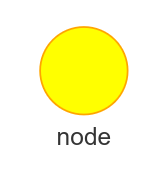
\includegraphics[width=0.7\textwidth]{figures/connecting_nodes/legend/node}
    \caption{Regular node created by the \ac{halgorithm}.\newline}%
    \end{subfigure}
    \begin{subfigure}{0.2\textwidth}
    \centering
    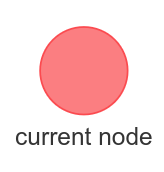
\includegraphics[width=0.7\textwidth]{figures/connecting_nodes/legend/current_node}
    \caption{Current node indicates that it's outgoing edge is now or is next to be executed.}%
    \end{subfigure}
    \begin{subfigure}{0.2\textwidth}
    \centering
    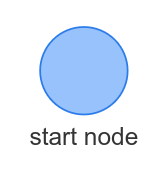
\includegraphics[width=0.7\textwidth]{figures/connecting_nodes/legend/starting_node}
    \caption{Starting node, one is generated at for every subtask.}%
    \end{subfigure}
    \begin{subfigure}{0.2\textwidth}
    \centering
    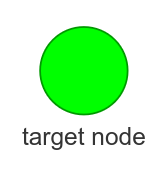
\includegraphics[width=0.7\textwidth]{figures/connecting_nodes/legend/target_node}
    \caption{Target node, one is generated for every subtask.\newline}%
    \end{subfigure}

    \begin{subfigure}{0.33\textwidth}
    \centering
    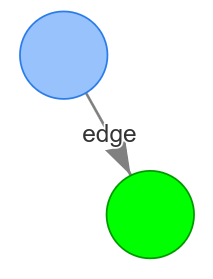
\includegraphics[width=0.7\textwidth]{figures/connecting_nodes/legend/edge}
    \caption{Edge with status IN, PE, SM, PP or EX.}%
    \end{subfigure}
    \begin{subfigure}{0.33\textwidth}
    \centering
    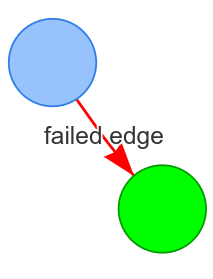
\includegraphics[width=0.7\textwidth]{figures/connecting_nodes/legend/failed_edge}
    \caption{Edge with status FAILED (FAIL)}%
    \end{subfigure}
    \begin{subfigure}{0.33\textwidth}
    \centering
    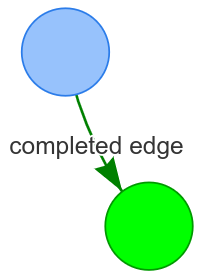
\includegraphics[width=0.7\textwidth]{figures/connecting_nodes/legend/completed_edge}
    \caption{Edge with status COMPLETED (CO)}%
    \end{subfigure}
    \caption{Legend for \ac{hgraph}'s nodes an edges}%
    \label{fig:hgraph_legend}
\end{figure}

\paragraph{Driving and Pushing} Four examples are presented, starting with a driving task in \cref{fig:robot_drive_hgraph}, then a pushing task in \cref{fig:robot_push_hgraph}.\bs

\begin{figure}[H]
    \centering
    \begin{subfigure}{.3\textwidth}
    \centering
    \includegraphics[width=0.7\textwidth]{figures/connecting_nodes/robot_to_target/robot_to_target}
    \end{subfigure}
    \begin{subfigure}{.3\textwidth}
    \centering
    \includegraphics[width=0.9\textwidth]{figures/connecting_nodes/robot_to_target/robot_drive_target}
    \end{subfigure}
    \begin{subfigure}{.3\textwidth}
    \centering
    \includegraphics[width=\textwidth]{figures/connecting_nodes/robot_to_target/robot_iden_drive_target}
    \end{subfigure}
    \caption{\ac{hgraph} generated by the \ac{halgorithm} to drive the robot to a target configuration}%
    \label{fig:robot_drive_hgraph}
\end{figure}

The robot does not have a system model of itself, thus first system identification must be performed before it can drive to the specified target configuration. The \ac{kgraph} that will be discussed in \cref{subsec:kgraph_definition} can suggest an action that includes a system model. In that case, system identification is not needed. The following figure displays succesfully executing the hypothesis found in \cref{fig:robot_drive_hgraph}.\bs

\begin{figure}[H]
    \centering
    \begin{subfigure}{.3\textwidth}
    \centering
    \includegraphics[width=0.8\textwidth]{figures/connecting_nodes/robot_to_target/execute_robot_to_target_1}
    \end{subfigure}
    \begin{subfigure}{.3\textwidth}
    \centering
    \includegraphics[width=0.8\textwidth]{figures/connecting_nodes/robot_to_target/execute_robot_to_target_2}
    \end{subfigure}
    \begin{subfigure}{.3\textwidth}
    \centering
    \includegraphics[width=0.8\textwidth]{figures/connecting_nodes/robot_to_target/execute_robot_to_target_3}
    \end{subfigure}
    \caption{Executing the hypothesis found in \cref{fig:robot_drive_hgraph}.}
    \label{fig:execute_robot_to_target}
\end{figure}

Upcoming figure will display the hypothesis generated to push an object to a target position. Both generating a hypothesis and executing the hypothesis are intertwined, this is because certain information should first be collected from the environment before the full hypothesis can be generated. An example is the \textit{best\_push\_position} that can be found in \cref{subfig:robot_push_7,subfig:robot_push_8,subfig:robot_push_9}. The \textit{best\_push\_position} can be found after manipulation planning for the pushing edge is completed. For motion planning a system model is required, thus the corresponding system identification edge should be completed before manipulation planning can start, and than the \textit{best\_push\_position} can be determined.\bs

\begin{figure}[H]
    \centering
    \begin{subfigure}{.3\textwidth}
    \centering
    \includegraphics[width=0.8\textwidth]{figures/connecting_nodes/robot_push/robot_push_1}
    \caption{}
    \end{subfigure}
    \begin{subfigure}{.3\textwidth}
    \centering
    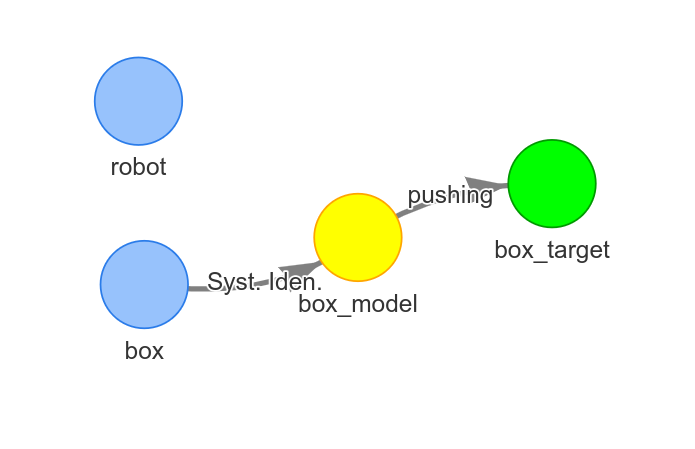
\includegraphics[width=1.1\textwidth]{figures/connecting_nodes/robot_push/robot_push_2}
    \caption{}\label{subfig:robot_push_2}
    \end{subfigure}
    \begin{subfigure}{.3\textwidth}
    \centering
    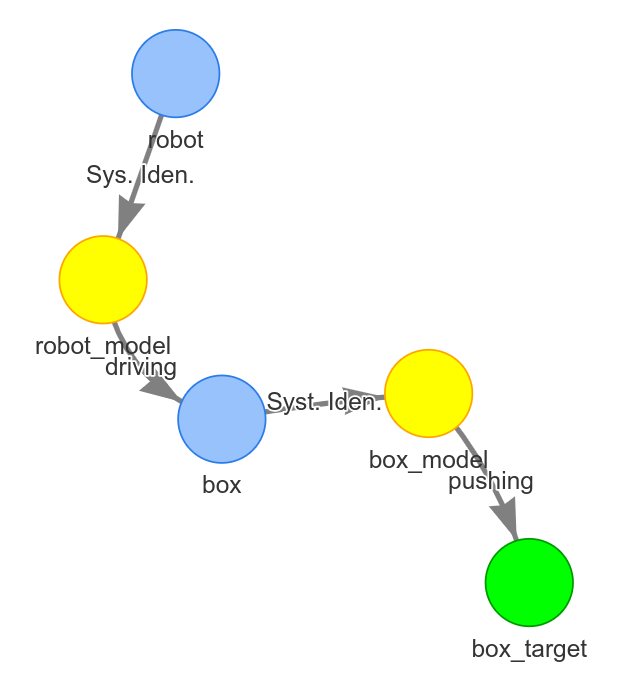
\includegraphics[width=1\textwidth]{figures/connecting_nodes/robot_push/robot_push_3}
    \caption{}\label{subfig:robot_push_3}
    \end{subfigure}

    \begin{subfigure}{.3\textwidth}
    \centering
    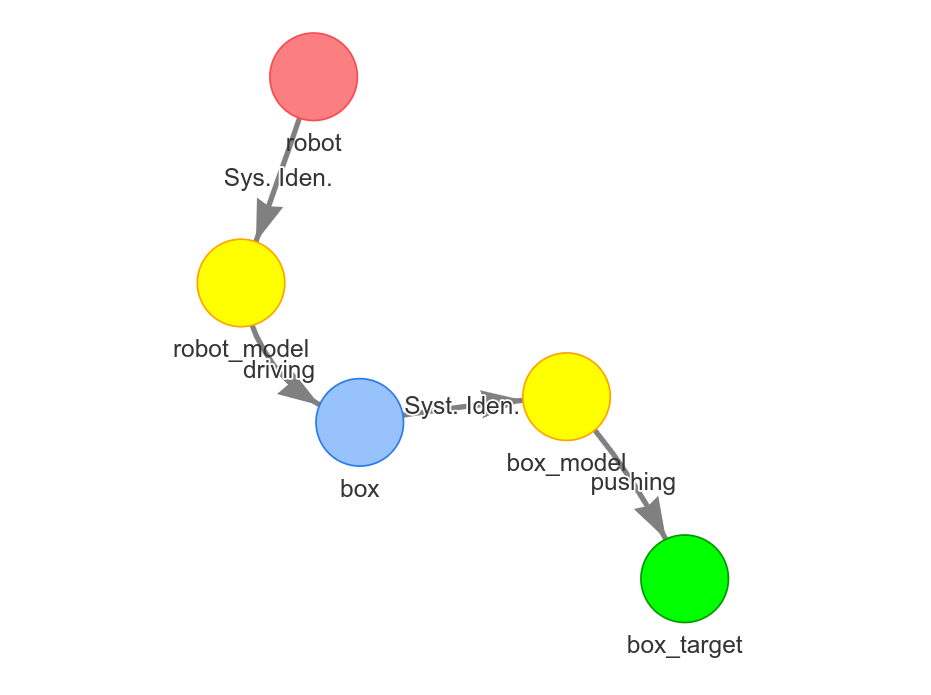
\includegraphics[width=1\textwidth]{figures/connecting_nodes/robot_push/robot_push_4}
    \caption{}\label{subfig:robot_push_4}
    \end{subfigure}
    \begin{subfigure}{.3\textwidth}
    \centering
    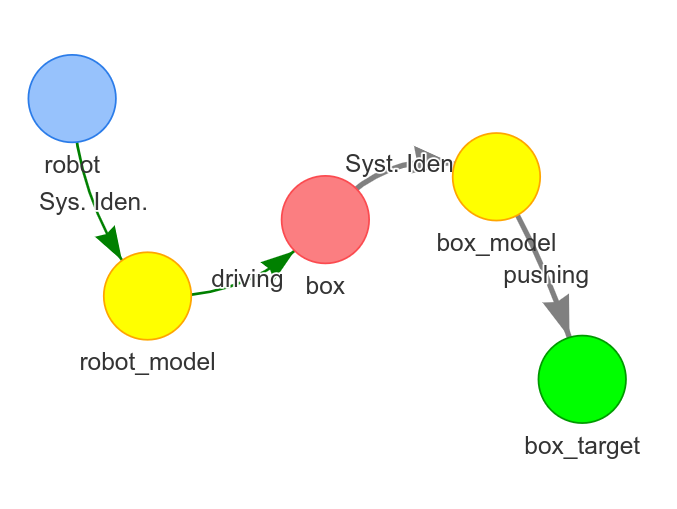
\includegraphics[width=1.05\textwidth]{figures/connecting_nodes/robot_push/robot_push_5}
    \caption{}\label{subfig:robot_push_5}
    \end{subfigure}
    \begin{subfigure}{.3\textwidth}
    \centering
    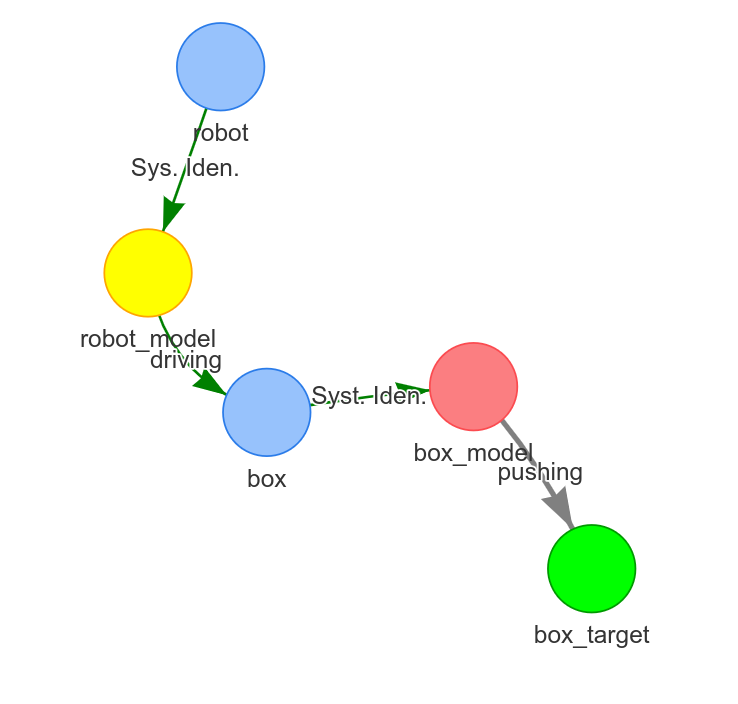
\includegraphics[width=1.05\textwidth]{figures/connecting_nodes/robot_push/robot_push_6}
    \caption{}\label{subfig:robot_push_6}
    \end{subfigure}

    \begin{subfigure}{.3\textwidth}
    \centering
    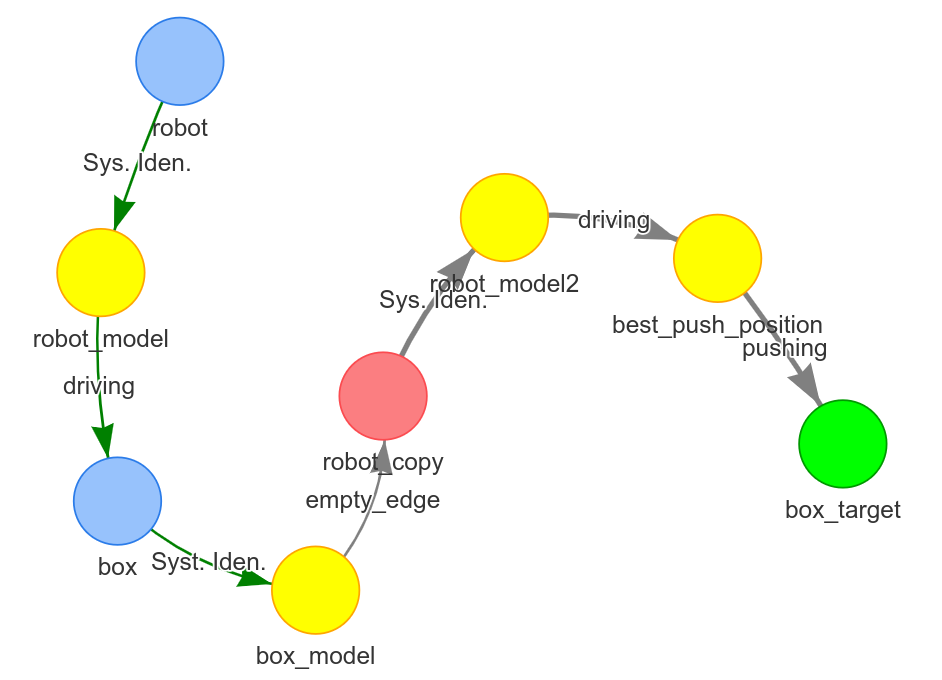
\includegraphics[width=1\textwidth]{figures/connecting_nodes/robot_push/robot_push_7}
    \caption{}\label{subfig:robot_push_7}
    \end{subfigure}
    \begin{subfigure}{.3\textwidth}
    \centering
    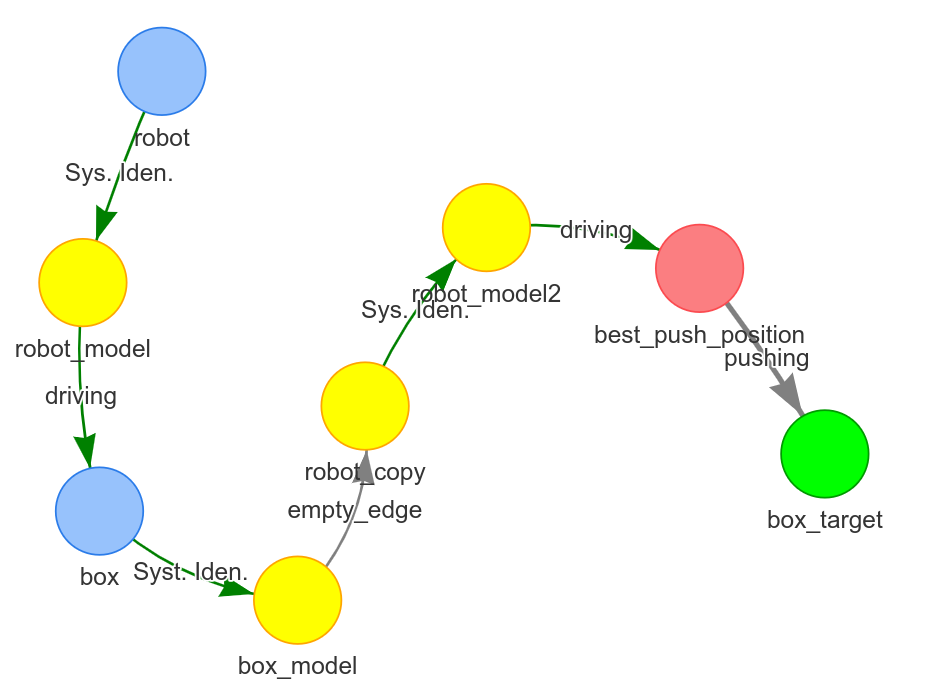
\includegraphics[width=1.05\textwidth]{figures/connecting_nodes/robot_push/robot_push_8}
    \caption{}\label{subfig:robot_push_8}
    \end{subfigure}
    \begin{subfigure}{.3\textwidth}
    \centering
    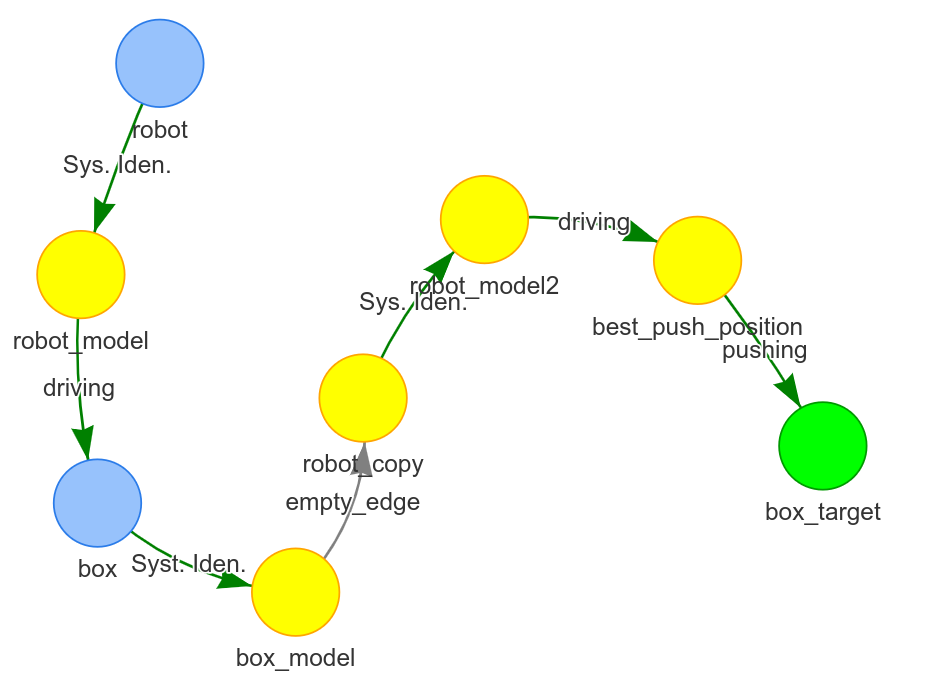
\includegraphics[width=1.05\textwidth]{figures/connecting_nodes/robot_push/robot_push_9}
    \caption{}\label{subfig:robot_push_9}
    \end{subfigure}
    \caption{\ac{hgraph} for pushing the green box to the target configuration}%
    \label{fig:robot_push_hgraph}
\end{figure}
Especially in \cref{subfig:robot_push_2,subfig:robot_push_3} the backward search is clearly visible, the \ac{halgorithm} searches from target node to the robot node. \Cref{fig:robot_push_hgraph} is extensive because every nessecary steps is included whilst some could be skipped. First, identifying a system model for robot driving twice, if the system model created in edge Sys. Iden. pointing toward node robot\_model is reused, then the edge Sys. Iden. pointing toward robot\_model\_1 would be unnecessary. Second, if system models would already be availeble for driving and pushing, no single system identification edge would be required. A \textit{empty\_edge} can be seen in \cref{subfig:robot_push_7,subfig:robot_push_8,subfig:robot_push_9}, the empty\_edge serves to connect a node to another node (box\_model to robot\_copy in \cref{fig:robot_push_hgraph}). The empty\_edge can be traversed without execution, holds no controller, system model or status.\bs

\paragraph{Encountering a Blocked Path}%
During propagation of an action edge's status, motion or manipulation planning occurs. If an object is blocking the path, planning will detect it and the \ac{halgorithm} tries to free the path. In the next example the \ac{halgorithm} detects a blocking object and frees the path by pushing the blocking object to a new configuration, and can be visulised in \cref{fig:blocking_obj_hgraph}.\bs

\begin{figure}[H]
    \centering
    \begin{subfigure}{.3\textwidth}
    \centering
    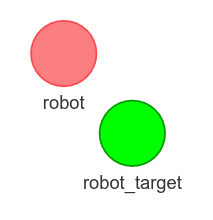
\includegraphics[width=0.5\textwidth]{figures/connecting_nodes/blocking_obj/blocking_obj_1}
    \caption{}
    \end{subfigure}
    \begin{subfigure}{.3\textwidth}
    \centering
    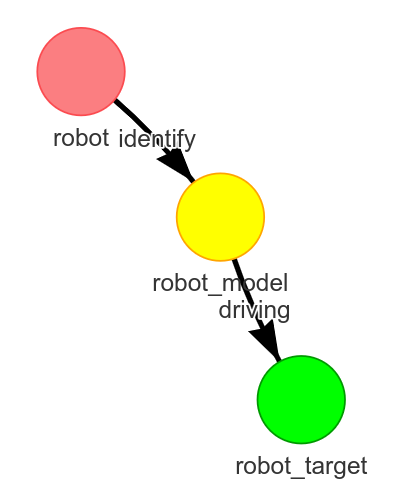
\includegraphics[width=\textwidth]{figures/connecting_nodes/blocking_obj/blocking_obj_2}
    \caption{}\label{subfig:blocking_obj_2}
    \end{subfigure}
    \begin{subfigure}{.3\textwidth}
    \centering
    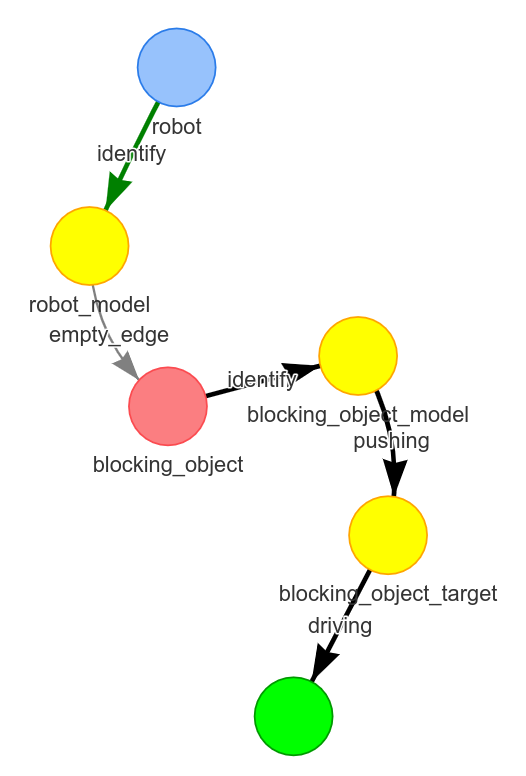
\includegraphics[width=\textwidth]{figures/connecting_nodes/blocking_obj/blocking_obj_3}
    \caption{}\label{subfig:blocking_obj_3}
    \end{subfigure}

    \begin{subfigure}{.3\textwidth}
    \centering
    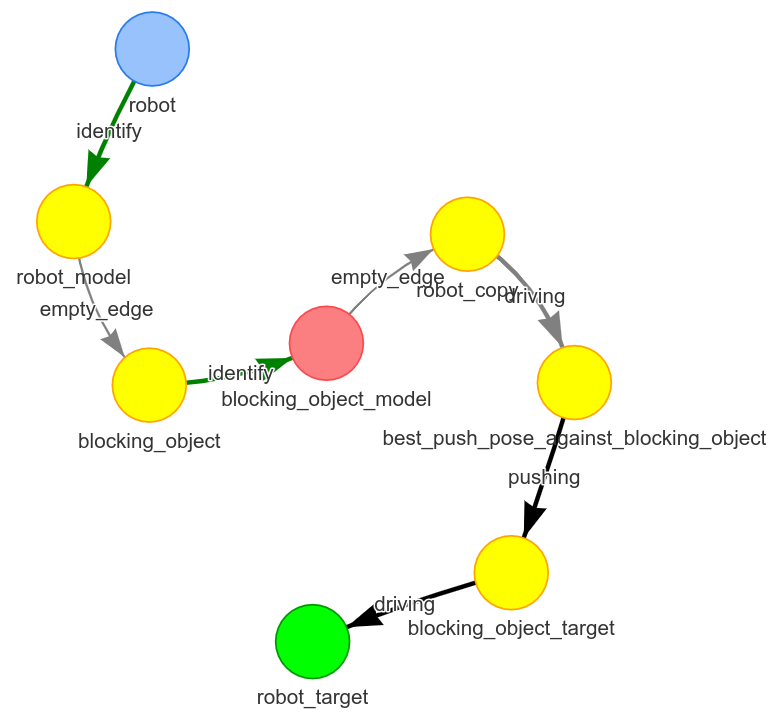
\includegraphics[width=1.3\textwidth]{figures/connecting_nodes/blocking_obj/blocking_obj_4}
    \caption{}\label{subfig:blocking_obj_4}
    \end{subfigure}
    \begin{subfigure}{.3\textwidth}
    \centering
    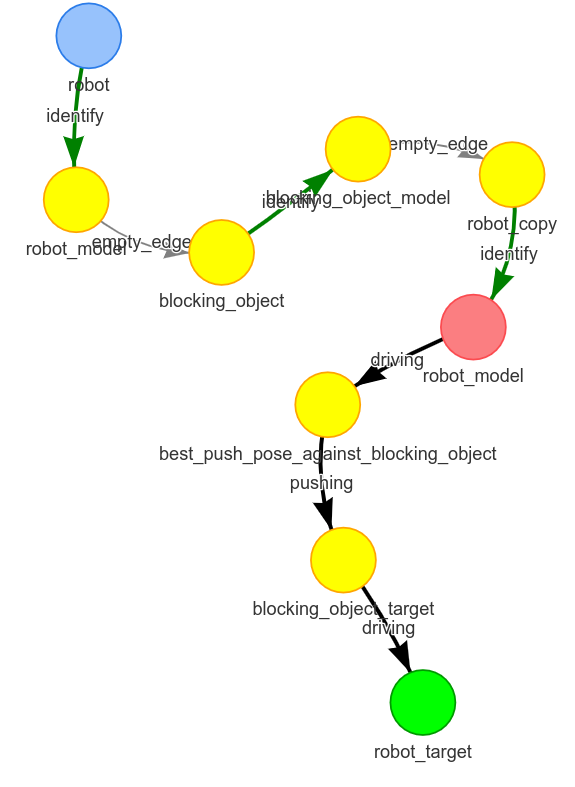
\includegraphics[width=\textwidth]{figures/connecting_nodes/blocking_obj/blocking_obj_5}
    \caption{}\label{subfig:blocking_obj_5}
    \end{subfigure}
    \begin{subfigure}{.3\textwidth}
    \centering
    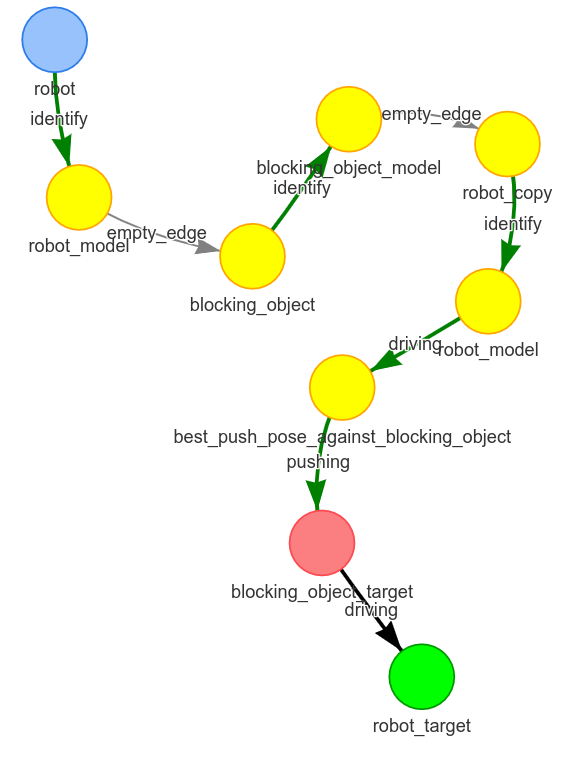
\includegraphics[width=\textwidth]{figures/connecting_nodes/blocking_obj/blocking_obj_6}
    \caption{}\label{subfig:blocking_obj_6}
    \end{subfigure}
    \caption{\ac{hgraph} for driving to target configuration and encountering a blocked path}%
    \label{fig:blocking_obj_hgraph}
\end{figure}

\paragraph{Encountering Failure}%
In the last example, the first hypothesis fails to complete and the \ac{halgorithm} tries to generate a new hypothesis that also fails to complete. Several faults and failures are modelled, the \ac{halgorithm} response to faults and failure is the same. If during the propagation of an edge's status any kind of failure arises, the failed edge and corresponding edges are marked as failed. Equally during execution, if a fault is detected, the execution halts and the edge and corresponding edges are marked as \quotes{failed}, the procedure can be seen in \cref{fig:failure_in_hgraph}.\bs

\begin{figure}[H]
    \centering
    \begin{subfigure}{.3\textwidth}
    \centering
    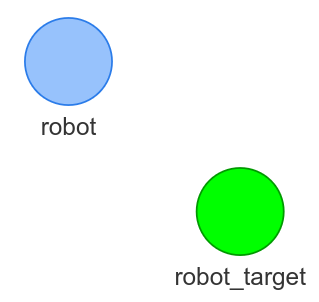
\includegraphics[width=0.8\textwidth]{figures/connecting_nodes/failure/fail_1}
    \end{subfigure}
    \begin{subfigure}{.3\textwidth}
    \centering
    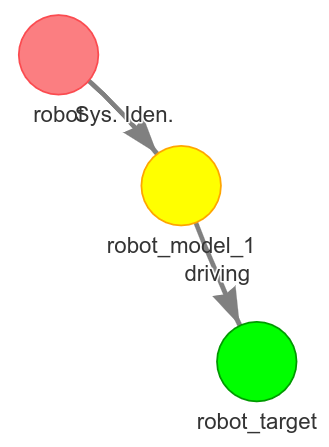
\includegraphics[width=1.1\textwidth]{figures/connecting_nodes/failure/fail_2}
    \end{subfigure}
    \begin{subfigure}{.3\textwidth}
    \centering
    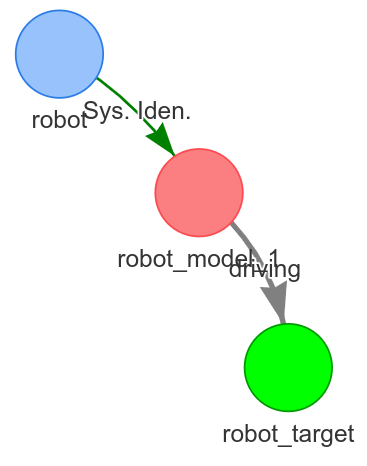
\includegraphics[width=1\textwidth]{figures/connecting_nodes/failure/fail_3}
    \end{subfigure}

    \begin{subfigure}{.3\textwidth}
    \centering
    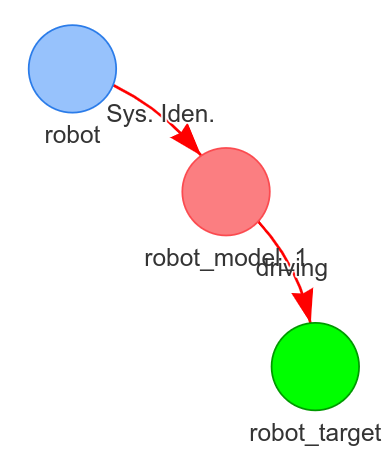
\includegraphics[width=1\textwidth]{figures/connecting_nodes/failure/fail_4}
    \end{subfigure}
    \begin{subfigure}{.3\textwidth}
    \centering
    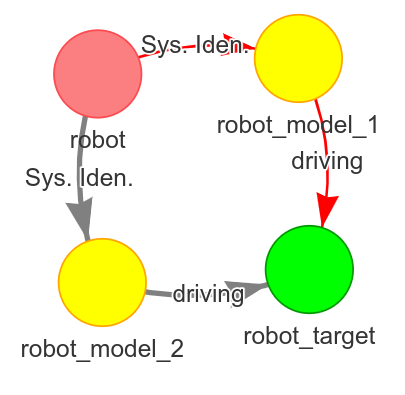
\includegraphics[width=1\textwidth]{figures/connecting_nodes/failure/fail_5}
    \end{subfigure}
    \begin{subfigure}{.3\textwidth}
    \centering
    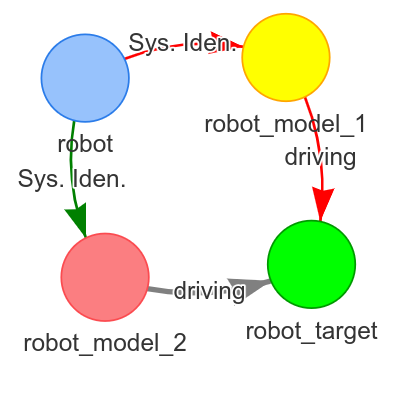
\includegraphics[width=1\textwidth]{figures/connecting_nodes/failure/fail_6}
    \end{subfigure}

    \begin{subfigure}{.3\textwidth}
    \centering
    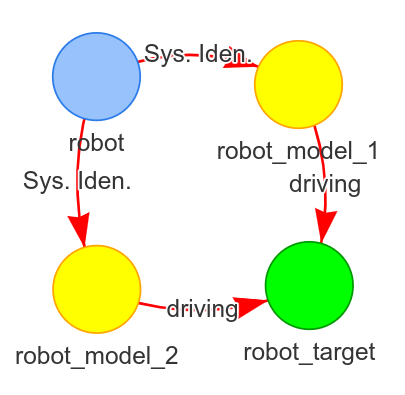
\includegraphics[width=1\textwidth]{figures/connecting_nodes/failure/fail_7}
    \end{subfigure}
    \hfill
    \caption{Executing two hypothesis, both failing to complete because a fault of failure emerged.}%
    \label{fig:failure_in_hgraph}
\end{figure}

In \cref{fig:failure_in_hgraph} only two parameterisations of drive controller and system model were available. Thus after two failed hypothesis the \ac{halgorithm} concludes it cannot complete this task.\bs


What by now hopefully became clear to the reader is that the \ac{hgraph} autonomously searches for hypotheses to solve the task, one subtask at a time. The \ac{hgraph} switches between the search and execution loop. Switching from the search loop toward the execution loop when a hypothesis is found, and switching back when a hypothesis is completed or an action failed to complete.\bs

The limited number of possible edges (every combination of a system identification method with a compatible control method) guarantees that the robot tries to connect 2 nodes, but concludes that it cannot reach a node if all possible edges have failed. Eventually running out of nodes to connect and conclude that a subtask cannot be completed.\bs

In the next section, the edges that are executed will be reviewed and stored in a knowledge base. The knowledge base will suggest edges when faced with similar nodes to connect.
\

\section{Hypothesis Algorithm}%
\label{sec:h-algorithm}
The \ac{h-algorithm} is the main component that orchestrates the actions and functions called to learn object properties and to complete a given task. This section starts with a simple example that generates and executes the hypothesis to drive toward a target pose. Then the search and execution loop are presented, that constitute the principal components of the proposed \ac{h-algorithm}. The terminology is elaborated upon step wise, whilst an example of a pushing task is discussed. Then two more examples are provided that allow to elaborate upon fault detection, the blocklist and the \ac{h-algorithm}'s response to a blocked path during task execution. Finally, the pseudocode can be resented, supported by a proposed \ac{h-algorithm} flowchart.\bs

Two arguments initialize the \ac{h-algorithm}, first, a set of object geometry that contains the dimensions of the objects in the robot environment for internal representation, and second a task to solve. Additionally several parameters must be specified, such as the grid size, maximum allowed input to the robot and tuning parameters for the path estimator, the path planner and controllers. When all arguments and parameters are provided, the \ac{h-algorithm} can be is initialized. There is only a single access point toward the \ac{h-algorithm}, the \textit{Respond(observation)} function. This function takes an environment \textit{observation} that updates the internal objects' poses. The function \textit{Respond($\cdot$)} returns control input for the robot. In this thesis, the sensor measurements coincide with the poses objects in the environment. Recall that the perfect-sensor assumption, assumption~\ref{assumption:perfect_object_sensor}, makes access to every object's exact configuration possible.\bs

Now a relatively simple example is presented to indicate how the \ac{h-algorithm} operates, later every step will be extensively elaborated. The example task consists of driving the robot object to a target pose. The leftmost subfigure in \cref{fig:robot_drive_h-graph} visualizes the initialization of a start and target node, which are connected with a drive action edge in the center figure. In the center subfigure, a system model must be provided to the controller that resides in the drive action edge. Motivating the \textit{sys. iden} edge and the $\gls{c}_\textit{robot\_model}$ node in the rightmost subfigure.\bs

\begin{figure}[h]
    \centering
    \begin{subfigure}{.3\textwidth}
    \centering
    \includegraphics[width=0.7\textwidth]{figures/proposed_method/connecting_nodes/robot_to_target/robot_to_target}
    \end{subfigure}
    \begin{subfigure}{.3\textwidth}
    \centering
    \includegraphics[width=0.9\textwidth]{figures/proposed_method/connecting_nodes/robot_to_target/robot_drive_target}
    \end{subfigure}
    \begin{subfigure}{.3\textwidth}
    \centering
    \includegraphics[width=\textwidth]{figures/proposed_method/connecting_nodes/robot_to_target/robot_iden_drive_target}
    \end{subfigure}
    \caption{First stages of the \ac{h-graph} when the \ac{h-algorithm} searches for an hypothesis to complete a driving task.}%
    \label{fig:robot_drive_h-graph}
\end{figure}

Now that an hypothesis is created that consists of an identification- and an action edge, the \ac{h-algorithm} alternates from the search loop to the execution loop, both loops are addressed shortly. The generated and executed example for a driving task just discussed is provided to show a simple example. It leaves many details out, which are now elaborated. Start with initializing start- and target nodes, then the search- and execution loop are discussed.\bs

\paragraph{Initialization of the \ac{h-algorithm}}
The \ac{h-algorithm} is initialized with a task that consists of one or more subtasks. Start- and target nodes are created for every subtask, and their status is set to INITIALIZED. Then the goal of the \ac{h-algorithm} is to connect every starting node to its corresponding target node with a hypothesis. The target node's status is set to COMPLETED when a hypothesis is completed successfully. If the \ac{h-algorithm} could not find a hypothesis that completes a subtask, the \ac{h-algorithm} concludes it cannot complete that subtask, and the target node's status is set to FAILED.\bs

\begin{figure}[H]
    \centering
    \begin{subfigure}{.3\textwidth}
    \centering
    \includegraphics[width=0.9\textwidth]{figures/proposed_method/connecting_nodes/robot_to_target/execute_robot_to_target_1}
    \end{subfigure}
    \begin{subfigure}{.3\textwidth}
    \centering
    \includegraphics[width=0.9\textwidth]{figures/proposed_method/connecting_nodes/robot_to_target/execute_robot_to_target_2}
    \end{subfigure}
    \begin{subfigure}{.3\textwidth}
    \centering
    \includegraphics[width=0.9\textwidth]{figures/proposed_method/connecting_nodes/robot_to_target/execute_robot_to_target_3}
    \end{subfigure}
    \caption{Multiple stages of the \ac{h-graph} when the \ac{h-algorithm} executes the hypothesis found in \cref{fig:robot_drive_h-graph}.}
    \label{fig:execute_robot_to_target}
\end{figure}

\subsection{The Search and the Execution Loop}
The proposed algorithm comprises two main parts, a search loop and an execution loop. The \ac{h-algorithm} searches for a hypothesis in the search loop. In the execution loop, the \ac{h-algorithm} tests hypotheses by executing the edges that form the hypothesis. A flowchart  of the \ac{h-algorithm} is presented at the very end of this chapter in \cref{tikz:flowchart_h-algorithm}, that flowchart will be familiar compared to the following figure, where the two main loops can be identified.\bs

\begin{figure}[H]
    \centering
    \includegraphics[width=7cm]{figures/proposed_method/two_loops_identified}
  \caption{The search (upper) and execution (lower) loop, that make up the main part of the proposed \ac{h-algorithm}. The figure's goal is to present the two loops, the flowchart in the background is presented full page in \Cref{tikz:flowchart_h-algorithm}.}%
    \label{fig:two_loops_identified}
\end{figure}

Hypotheses are formed while the \ac{h-algorithm} resides in the search loop. Forming a hypothesis generates nodes, edges, and progressing their status as described in \cref{tikz:status_identification_edge,tikz:status_action_edge}. In the execution loop \textit{an edge is being executed}, a phrase to describe that the controller residing in an edge is sending control input toward the robot. The \ac{h-algorithm} operates synchronously. The result is that the robots cannot operate whilst the \ac{h-algorithm} resides in the search loop, and during execution, no hypothesis can be formed or updated. The execution loop executes the edges that form the hypothesis one by one until either a fault is detected or the hypothesis is completed. Upon fault or completion, the \ac{h-algorithm} alternates back to the search loop\bs

When entering or re-entering the search loop, the first thing to determine is if there are unfinished subtasks and, if unfinished subtasks exist, which nodes to connect in order to form a hypothesis that completes that subtask. For such functionality three functions are created; \textit{SubtaskNotFinished}, \textit{GoBackward(\gls{node})}, \textit{FindCorrespondingNode(\gls{node})}. These functions are now discussed.\bs

\paragraph{Finding unfinished subtasks}
Determining if there exists an unfinished subtask is validated with the \textit{SubtaskNotFinished(\gls{task})} function. It checks the status for every target node in \ac{h-graph}. The three statuses are; INITIALIZED, COMPLETED and FAILED. A target node with an INITIALIZED status corresponds to an uncompleted subtask and is returned by the \textit{SubtaskNotFinished(\gls{task})} function. If all existing target nodes have either a completed or failed status, the \ac{h-algorithm} concludes that the task is completed.\bs

The \ac{h-algorithm} relies on a backward search technique, which can be described as: \textit{start the search at a goal state and work backwards until the initial state is encountered~\cite{lavalle_planning_2006}.} A motivation for a backward search over a forward search is that it might be the case that the branching factor is significant when starting from the initial state. In such cases, it might be more efficient to use a backward search. If the \textit{SubtaskNotFinished} returns an unfinished subtask, the \ac{h-algorithm} starts searching for a hypothesis connecting the start node to the corresponding target node. The first step is to find the right nodes in the \ac{h-graph}, which is now discussed.\bs

\paragraph{Creating a hypothesis for a subtask}
The \textit{SubtaskNotFinished} returns a target node corresponding to a unfinished subtask. Then if a subtask is unfinished, the \ac{h-algorithm} starts searching for a hypothesis connecting the start node to the target node. In \cref{subfig:robot_push_1}, the nodes to connect are the $\gls{node}_\mathit{box}$ node to the $\gls{node}_\textit{box\_target}$ node. These two nodes are a start- and a target node, the nodes to connect are not necessarily start- and target nodes themselves, as seen in \cref{subfig:robot_push_2}. Here the $\gls{node}_\textit{robot}$ node must be connected to the $\gls{node}_\textit{box}$ node. These nodes are both starting nodes. The first challenge is to find the two nodes to connect from an unfinished target node.\bs

The \textit{GoBackward($\gls{node}_\mathit{target}$)} function takes a target node $\gls{node}_\mathit{target}$ that corresponds to a unfinished subtask. It then traverses backwards via non-failed edges. The function stops traversing back when it encounters a node with a FAILED status or when no non-failed edge exists to traverse backwards over. The \textit{GoBackward} function thus finds a node, that node points toward the target node over a sequence of edges with a status other than failed, and all these edges point toward nodes with a status other than failed. In \cref{subfig:robot_push_1} the \textit{GoBackward($\gls{node}_\mathit{box\_target})$} function returns the $\gls{node}_\mathit{box\_target}$ node, in \cref{subfig:robot_push_2} the \textit{GoBackward($\gls{node}_\mathit{box\_target})$} returns the $\gls{node}_\mathit{box}$ node.\bs

The \textit{GoBackward($\gls{node}_\mathit{target}$)} finds a node to connect to, a corresponding node is sought to connect from. The \textit{FindCorrespondingNode(\gls{node})} finds a corresponding node to connect from. \textit{FindCorrespondingNode(GoBackward(\gls{node}))} takes a node as parameter and returns an existing node that contains the same object as its arguments node; if such a node does not exist, a new node is created.
\[\gls{node}_\mathit{to} =  \mathit{GoBackward(\gls{node}_\mathit{target})}\]
\[\gls{node}_\mathit{from} = \mathit{FindCorrespondingNode(GoBackward(\gls{node}_\mathit{target}))}\]

When elaborating the \ac{h-algorithm}, an example presents a visual example with every step in the \ac{h-algorithm}. In this example, the robot generates a hypothesis to complete a pushing task that contains a single subtask, initialization and the first generated edges are presented in \cref{fig:robot_push_1}.\bs

\begin{figure}[h]
    \centering
    \begin{subfigure}{.3\textwidth}
    \centering
    \includegraphics[width=0.9\textwidth]{figures/proposed_method/connecting_nodes/robot_push/robot_push_1}
    \caption{Initialize start- and target nodes.}\label{subfig:robot_push_1}
    \end{subfigure}
    \begin{subfigure}{.32\textwidth}
    \centering
    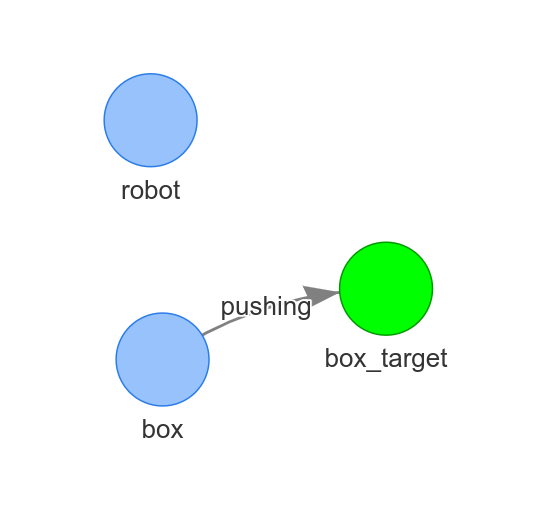
\includegraphics[width=\textwidth]{figures/proposed_method/connecting_nodes/robot_push/robot_push_2_new}
    \caption{Creation of a push action edge.}\label{subfig:robot_push_2}
    \end{subfigure}
    \begin{subfigure}{.35\textwidth}
    \includegraphics[width=1.2\textwidth]{figures/proposed_method/connecting_nodes/robot_push/robot_push_2}
    \caption{Creation of a identification edge.}\label{subfig:robot_push_3}
    \end{subfigure}
    \caption{First stages of the \ac{h-graph} when the \ac{h-algorithm} creates an hypothesis for a pushing task.}%
    \label{fig:robot_push_1}
\end{figure}

\paragraph{Creating edges}
The \textit{ConnectWithEdge($\gls{node}_1, \gls{node}_2$)} function connects two nodes with an edge, such as the nodes $\gls{node}_\mathit{from}, \gls{node}_\mathit{to}$ just introduced. It is required that both nodes contain the same object. The push action edge generated and displayed in \cref{subfig:robot_push_2} is between two nodes containing the \textit{box} object.\bs

Pushing edges must satisfy pre-conditions that cannot reside in the pushing edge itself. Thus pushing edges also they spawn new nodes by default. The robot must first drive toward a push pose against or close to the object to push. When a push action edge has planned a path, and updates its status to PATH IS PLANNED, the \ac{h-algorithm} then creates a $\gls{node}_\mathit{best\_push\_position}$ node, which configuration depends on the object's planned path. Thus, a path is planned for the push action, and then the best push pose is determined. The newly created node is connected before the push action edge, where an empty edge points from $\gls{node}_\mathit{best\_push\_position}$ to $\gls{edge}_\mathit{drive}$'s source node. The first occurrence of an $\gls{node}_\mathit{best\_push\_position}$ can be visualized in \Cref{subfig:robot_push_4}.\bs

\paragraph{Classifying objects}
When it is unknown if objects are movable or unmovable, a push action edge performs a tests to determine the class of an object. If the push action is unable to move the object in the first 50 time steps, the object is classified as UNMOVABLE, otherwise it is classified as MOVABLE.\bs

\paragraph{Valid Hypotheses}
Before a hypothesis can be executed, the hypothesis must be valid. A hypothesis is valid when two conditions are met. First, the hypothesis starts at the start node and points toward the target node over a sequence of successive edges with a non-failing status. Second, the first edge in the hypothesis must be ready for execution which the next paragraph will elaborate upon further. To indicate a node or edge has a status other than the FAILED status, that node or edge is called a non-failed node or -edge. To check if an hypothesis is valid the \textit{IsConnected($\gls{node}_1, \gls{node}_2$)} is created. This function checks if there exists a path in the \ac{h-graph} from $\gls{node}_1$ to $\gls{node}_2$ over a sequence of non-failing nodes and -edges. In the pushing task example, the first occurrence of a valid hypothesis is presented in \Cref{subfig:robot_push_4}.\bs

An \textit{EmtpyEdge} is introduced to involve nodes that contain different objects. The emptyEdge serves only to connect nodes that contain different objects and can have status INITIALIZED or FAILED. The \ac{h-algorithm} can traverse over emptyEdge if the status is INITIALIZED.\bs

\begin{figure}[H]
    \centering
    \begin{subfigure}{.45\textwidth}
    \centering
    \includegraphics[width=1\textwidth]{figures/proposed_method/connecting_nodes/robot_push/robot_push_4_new}
    \caption{Executing the hypothesis and generated new nodes.}\label{subfig:robot_push_4}
    \end{subfigure}
    \begin{subfigure}{.45\textwidth}
    \centering
    \includegraphics[width=1\textwidth]{figures/proposed_method/connecting_nodes/robot_push/robot_push_5_new}
    \caption{Executing the pushing edge.}\label{subfig:robot_push_5}
    \end{subfigure}
    \caption{The hypothesis for a pushing task becomes valid and is executed. Then a path for the pushing edge\\is planned which generates new nodes to drive toward the best push pose against the box.}%
    \label{fig:robot_push_2}
\end{figure}

\paragraph{Preparing edges for Execution}
In contrast to identification edges, action edges must first take several actions in preparation before they are ready to send input toward the robot. The status of an edge indicates at which step of preparing the action edge is and can be visualized in \Cref{tikz:status_action_edge}. After initialization, the action edge performs path estimation, loads in a system model, performs path planning and then, it is ready for execution. Two functions are created to make edges ready for execution. The \textit{ReadyForExecution(\gls{edge})} validates if an edge is ready for execution. Identification edges are ready for execution when they bear a non-failed status, action edges are ready for execution when they bear the PATH PLANNED or EXECUTING status. The \textit{MakeReady(\gls{edge})} function takes an edge and takes action depending on its status presented in the following table.\bs

\begin{table}[H]
    \caption{The action edge status is presented in the left column, the corresponding action taken by the \textit{MakeReady} function to prepare an action edge for execution in the right column. An action edge increments its status as indicated in \Cref{tikz:status_action_edge}.}%
    \label{table:make_action_edge_ready}
    \centering
    \begin{tabular}%
    {>{\raggedright\arraybackslash}p{0.25\textwidth}|%
    >{\raggedright\arraybackslash}p{0.65\textwidth}}
      Action edge status& action taken by \textit{MakeReady} function\\\toprule
      INITIALIZED& Create a path estimator and estimate path existence. If no path can be estimated, the status is updated to FAILED. If a path can be estimated, a shortest path is found that acts as a \quotes{warm start} for the path planner.\\
      PATH EXISTS& Load in a system model.\\
      SYSTEM MODEL& Create path planner and plan path. The edge status is updated to FAILED if no path can be found. If a path is found, it acts as a reference signal for the controller. In the case of an push action edge, a $\gls{node}_\mathit{best\_push\_position}$ is created. Additionally, the path the planner finds can indicate that an object is blocking. In such cases, the \ac{h-algorithm} must first push that object to free the path. An example of such a case is provided in \Cref{fig:blocking_obj_h-graph_one}.
    \end{tabular}
\end{table}

\paragraph{Hypothesis Execution}
When the \ac{h-algorithm} creates a valid hypothesis, it switches from the search loop to the execution loop. Executing a hypothesis is managed by three functions. The first edge in the hypothesis is ready for execution and thus contains a controller and a path to track. That edge is executed, and its controller sends input toward the robot to track the path. The \textit{SteerTowardTarget(\gls{edge})} calculates the input that steers the robot toward the path. The \textit{TargetNotReached(\gls{edge})} validates if the robot has reached the target, which is the last configuration in the path. A margin is set by which the \textit{TargetNotReached(\gls{edge})} concludes that the robot is close enough to the final target pose. For drive actions, that margin is set to 0.1 meters measured in Euclidean instance between the robot and the robot's target position.

For push action, that margin is set to 2 meters, measured in Euclidean distance between the object and the object's target position. These values are tuned by trial and error and is one of the improvements that can be made in future work. The large margin for pushing tasks is set to ensure that the target pose is reached. With a lower margin, the object is often pushed further than the target position. A fault is then detected because the deviated too much from the path, the robot then drives toward the object's opposite side to again, push it over the target position. Fault detection is discussed in upcoming paragraph. After the successful completion of an edge, the next edge in the hypothesis is selected by the \textit{IncrementEdge} function. Two possible outcomes exist, the next edge is ready for execution, then the \ac{h-algorithm} remains in the execute loop. Or, the next edge is not yet ready, then the \ac{h-algorithm} goes from the execution loop toward the search loop to prepare the next edge for execution.\bs

\begin{figure}[H]
    \centering
    \includegraphics[width=0.5\textwidth]{figures/proposed_method/connecting_nodes/robot_push/robot_push_6}
    \caption{The \ac{h-graph} after the pushing task was successfully completed.}%
    \label{fig:robot_push_5}
\end{figure}

\paragraph{Completing Hypotheses and Edges}
When the last edge in an hypothesis is completed, that subtask is completed. The \ac{h-graph} randomly selects a next subtask to complete until there are no unfinished subtasks left, the \ac{h-algorithm} then concludes that the task is completed. Opposed to successful completion, subtasks can unsuccessfully complete, which is discussed in the upcoming paragraph.\bs

\subsection{Fault Detection}%
\label{sec:monitoring_metrics}
The proposed framework implements a fault metric named the \textit{monitored metrics} which are presented shortly, first motivation for the monitoring metrics is given. When the \ac{h-algorithm} resides in the execution loop, it cannot search for action sequences, which is performed in the search loop. During the execution of an action, the \acl{h-algorithm} is unable to perform any other action. This blocking behavior has some implications, mainly that the controller can steer the system to a configuration from which it cannot independently reach the target configuration, as a result, it will never halt. For example, a controller tries to drive the robot toward a target configuration but there is an unmovable obstacle in the way. Another example is the controller is closed-loop unstable and never reaches its target configuration. Both examples do not occur is well defined simulation environments, because of the \textit{closed-world assumption}. In the real world, an unexpected blocking obstacle or unstable controllers are more likely to occur.\bs

Detecting controller faults is a large robotic topic~\cite{khalastchi_fault_2019}, properly implementing a fault detection and diagnosis module is out of the scope of this thesis. Instead, two simple metrics will be monitored during execution, by the \textit{FaultDetected(\gls{edge})} function. Upon detection of a fault, the \textit{HandleFault(\gls{edge})} function then updates the executing edge's status to FAILED, and the \ac{h-algorithm} switches from the execution loop to the search loop in search for a new hypothesis. The first monitoring metric is \acl{PE}, and can be described as:\\
With the current configuration of the system, calculated system input and a system model, a prediction info the future is made every time step. Then the system input is applied to the system, the time step incremented and the configuration is measured. The prediction error is than the difference between predicted and measured configuration.\bs

The \ac{PE} is defined as:

\[ \gls{pe}(\gls{k}) ::= ||\gls{Cest}(\gls{k}|\gls{k}-1) - \gls{c}(\gls{k})|| \]

Where $\gls{Cest}(\gls{k}|\gls{k}-1)$ is a prediction of the configuration and $\gls{c}(\gls{k})$ is the measured configuration.\bs

During execution a sudden high \ac{PE} indicates unexpected behavior occurs, such as when the robot has driven into an object which it was not expecting. A high \ac{PE}, which persists indicates that the robot is continuously blocked. A few high prediction errors are allowed, but when the \ac{PE} exceeds a pre-defined threshold and persists over a pre-defined time, the \ac{h-graph} concludes that there was an fault detected during execution and the edge's status is updated to FAILED.\bs

The second monitoring metric is the \acl{TE} that can be described as:\\ A controller tracks a path that consists of a list of configurations by steering the system to the upcoming configuration in the list. When that configuration is reached, the upcoming configuration is updated to the next configuration in the path. The \ac{TE} is the difference between the current configuration of the system and the upcoming configuration.\bs

The \ac{TE} is defined as:

\[ \gls{te}(\gls{k}) ::= ||\gls{c}_\mathit{upcoming} - \gls{c}(\gls{k})|| \]

Where $\gls{c}_\mathit{upcoming}$ is the target configuration in the path that the controller tries to steer toward, and \gls{c}(\gls{k}) is the measured configuration.\bs

The system should not diverge too far from to path it is supposed to track, if the robot diverges more than a pre-defined threshold the \ac{h-graph} concludes that there was an error during execution and the edge fails. $\gls{c}_\mathit{upcoming}$ does not update every time step, whilst \gls{c}(\gls{k}) does update every time step. As a result, a \quotes{good} \ac{TE} is expected to take the form of a saw tooth function inverted over the horizontal x-axis.\bs

The predefined thresholds are split for drive and push actions because driving actions have much lower average \ac{PE} and \ac{TE} compared to push actions. For drive action edges, when the average of the last 25 recorded \ac{PE}'s is higher than 0.05 meter, or the \ac{TE} is higher than 2 meters, a fault is concluded. For push actions only a \ac{TE} is used, which is split into two parts. One ensures the object follows the path, and another ensures that the robot does not deviate too far from the object. If, for a pushing edge, the object deviates more than 2 meters from the path or the robot deviates more than 2 meters from its push position determined by the object pose, a fault is concluded.\bs

\subsection{The Blocklist}%
The blocklist prevents the regeneration of failed edges. The infinite loop of creating an edge that fails only to be regenerated is prevented. The blocklist keeps a list of edge parameterization as well as the node identifier if failed on. Newly generated edges are checked against this blocklist, if they are on the blocklist, initialization of the edge is prevented. The possible parameterizations are filtered when two nodes are connected with an action edge. Thus, any parameterization on the blocklist for a specific node (to which the action edge would point to) cannot be created again for the lifetime of the \ac{h-graph}.\bs

In the following example, \Cref{fig:failure_in_h-graph} faults are detected, these edges are added to the blocklist, the first hypothesis fails to complete, and the \ac{h-algorithm} tries to generate a new hypothesis that also fails to complete.\bs

\begin{figure}[H]
    \centering
    \begin{subfigure}{.3\textwidth}
    \centering
    \includegraphics[width=\textwidth]{figures/proposed_method/connecting_nodes/failure/fail_2}
    \end{subfigure}
    \begin{subfigure}{.3\textwidth}
    \centering
    \includegraphics[width=\textwidth]{figures/proposed_method/connecting_nodes/failure/fail_3}
    \end{subfigure}
    \begin{subfigure}{.3\textwidth}
    \centering
    \includegraphics[width=\textwidth]{figures/proposed_method/connecting_nodes/failure/fail_4}
    \end{subfigure}

    \begin{subfigure}{.3\textwidth}
    \centering
    \includegraphics[width=1\textwidth]{figures/proposed_method/connecting_nodes/failure/fail_5}
    \end{subfigure}
    \begin{subfigure}{.3\textwidth}
    \centering
    \includegraphics[width=1\textwidth]{figures/proposed_method/connecting_nodes/failure/fail_6}
    \end{subfigure}
    \begin{subfigure}{.3\textwidth}
    \centering
    \includegraphics[width=1\textwidth]{figures/proposed_method/connecting_nodes/failure/fail_7}
    \end{subfigure}
    \hfill
    \caption{Multiple stages of the \ac{h-graph}. The two hypotheses both failed during execution because a fault was detected. The failed edges are added to the blocklist, preventing the regeneration of edges with the same parameterization. The \ac{h-algorithm} concludes the task to be unfeasible.}%
    \label{fig:failure_in_h-graph}
\end{figure}

In \Cref{fig:failure_in_h-graph}, only two parameterizations of drive controllers and system models were available. Thus after two failed hypotheses, the \ac{h-algorithm} concludes that the task is unfeasible. All functionality is now discussed and is neatly summarized in the following table. Then, pseudocode for the proposed \ac{h-algorithm} is presented.\bs

\subsection{Encountering a Blocked Path}%
During the propagation of an action edge's status, path planning occurs discussed in \Cref{subsec:path_planning,chap:proposed_planning}. A blocking object is detected when the path found crosses through unknown of movable space. An example is now discussed that elaborates upon the \ac{h-algorithm} response when encountering a blocked path. An example of such an environment can be visualized in \Cref{subfig:push_or_drive_env} where the \textit{UnknownSpaceCost} is set to 0.5 meter. The example \ac{h-graph} that will now be discussed generalizes over drive tasks that can be completed if an blocking object is pushed to free the path.\bs

The \ac{h-algorithm} creates the start- and target node for the robot in \Cref{subfig:blocking_obj_1}, and creates a first hypothesis which can be visualized in \Cref{subfig:blocking_obj_2}. When propagating the drive action edge status, path planning occurs, during which a blocking object is detected that blocks a direct path. To free that path two nodes are generated, first, a target node for the blocking object \textit{blocking\_object\_target} that target node indicates the blocking object at a pose that is no longer blocking the path. The second node represents the blocking object at its current pose, because there does not yet exist a node for the blocking object at its current pose, the \ac{h-algorithm} generates a new node for the blocking object at it's current pose named \textit{blocking\_object} that can be seen in \Cref{subfig:blocking_obj_3}.\bs

\begin{figure}[H]
  \centering
  \begin{subfigure}{.3\textwidth}
    \centering
    \includegraphics[width=0.6\textwidth]{figures/proposed_method/connecting_nodes/blocking_obj/blocking_obj_1}
    \caption{}\label{subfig:blocking_obj_1}
  \end{subfigure}
  \begin{subfigure}{.3\textwidth}
    \centering
    \includegraphics[width=0.9\textwidth]{figures/proposed_method/connecting_nodes/blocking_obj/blocking_obj_2}
    \caption{}\label{subfig:blocking_obj_2}
  \end{subfigure}
  \begin{subfigure}{.3\textwidth}
    \centering
    \includegraphics[width=\textwidth]{figures/proposed_method/connecting_nodes/blocking_obj/blocking_obj_3}
    \caption{}\label{subfig:blocking_obj_3}
  \end{subfigure}

  \caption{Multiple stages of the \ac{h-graph} for a driving task, where an blocked path is encountered.}%
  \label{fig:blocking_obj_h-graph_one}

\end{figure}

The newly generated pushing edge between node \textit{blocking\_object\_model} and \textit{blocking\_object\_target} is initialized with a randomly selected controller. To fully parameterize the pushing edge a controller with a compatible system model is required. To generate a system model, the \ac{h-algorithm} generates a pushing identification edge and node \textit{blocking\_object\_model}.\bs

After identifying a system model that describes pushing against the blocking object, path planning for the blocked object from its current pose toward it's target pose occurs. The initial pose for the robot against the blocked object can then be determined because that initial pose is dependent on the planned path. \Cref{subfig:blocking_obj_4} displays the drive edge toward the best initial push pose indicated by the \textit{best\_push\_pose\_against\_blocking\_object} node. Equivalent to the generation of a blocking object node at its current pose in \Cref{subfig:robot_push_3}, a robot node is generated at the current robot's pose, named \textit{robot\_copy} in \Cref{subfig:blocking_obj_4}, because a node at the current robot pose did not yet exist. A drive edge is generated between the \textit{robot\_copy} and \textit{best\_push\_pose\_against\_blocking\_object} nodes. The identification edge is later generated as can be seen in \Cref{subfig:blocking_obj_5}.\bs

\begin{figure}[H]
    \centering
    \includegraphics[width=0.5\textwidth]{figures/proposed_method/connecting_nodes/blocking_obj/blocking_obj_4}
    \caption{Snapshot of the \ac{h-graph} during drive task, where a blocked path is encountered. The (red) current node indicates that next action is to drive toward the best push pose against the blocking object.}\label{subfig:blocking_obj_4}
\end{figure}

\Cref{subfig:blocking_obj_5,subfig:blocking_obj_6} visualize driving toward the best push pose against the blocking object, pushing the blocked object to its target pose, and finally driving toward the robots target pose.\bs

\begin{figure}[H]
  \centering
  \begin{subfigure}{.3\textwidth}
    \centering
  \includegraphics[width=\textwidth]{figures/proposed_method/connecting_nodes/blocking_obj/blocking_obj_5}
    \caption{}\label{subfig:blocking_obj_5}
  \end{subfigure}
  \begin{subfigure}{.3\textwidth}
    \centering
    \includegraphics[width=\textwidth]{figures/proposed_method/connecting_nodes/blocking_obj/blocking_obj_6}
    \caption{}\label{subfig:blocking_obj_6}
  \end{subfigure}
  \caption{\ac{h-graph} final stages before successfully completing a driving task, during which a blocked path is encountered.}%
  \label{fig:blocking_obj_h-graph_two}
\end{figure}

Now that the \ac{h-algorithm} is defined and discussed, pseudocode is presented. The following table summarizes the functions that will be used by the pseudocode in \Cref{pseudocode:h-algorithm}.\bs

\begin{table}[H]
\caption{The functions employed by the \ac{h-algorithm} in \Cref{pseudocode:h-algorithm}.}
\label{table:functions_for_h-algorithm}
\centering
\begin{tabular}%
  {>{\raggedright\arraybackslash}p{0.25\textwidth}%
   >{\raggedright\arraybackslash}p{0.65\textwidth}}
\textit{SubTaskNotFinished(\gls{subtask})}:& Return False if the subtask \gls{subtask} is completed or it is concluded to be unfeasible \\
\textit{IsConnected($\gls{node}_1, \gls{node}_2$)}:& Return True if there exist a path in the \ac{h-graph} from node $\gls{node}_1$  to node $\gls{node}_2$ through a number of non-failed edges\\
\textit{ReadyForExecution(\gls{edge})}: & Return True if the edge \gls{edge} is ready to execute\\
\textit{TargetNotReached(\gls{edge})}: & Return True edge \gls{edge} has not reached it target configuration\\
\textit{FaultDetected(\gls{edge})}: & Return True if a fault has been detected during execution of edge \gls{edge}\\

\textit{HandleFault(\gls{edge})}: & Update edge \gls{edge} status to FAILED and remove edge from hypothesis \\
\textit{SteerTowardTarget(\gls{observation})}: & Update controller with observation \gls{observation} and compute response that steers the system to target configuration\\
\textit{ReadyForExecution(\gls{edge})}: & Check if edge \gls{edge} has the PATH IS PLANNED status and contains all components to track the path\\
\textit{IncrementEdge}: & Mark current edge as completed, set next edge in \gls{hypothesis} as current edge if ready for execution, otherwise, enter search loop \\
\textit{MakeReady(\gls{edge})}: & Perform actions (see \Cref{table:make_action_edge_ready} for detailed information) to make the edge \gls{edge} ready for execution \\
\textit{GoBackward(\gls{node})}: & Find the source node that point toward \gls{node} through a number of non-failed edges\\
\textit{FindCorrespondingNode(\gls{node})}: & Find the node containing the same object as \gls{node} \\
\textit{ConnectWithEdge($\gls{edge}_1, \gls{edge}_2$)}: & Randomly generate edge between nodes $\gls{node}_1$ and $\gls{node}_2$ or use \ac{k-graph} to suggest an edge\\
\end{tabular}
\end{table}

\noindent
\begin{algorithm}[H]
  \caption{Pseudocode for the proposed hypothesis algorithm.}\label{pseudocode:h-algorithm}
  \begin{algorithmic}[1]

    \hspace{-0.9cm}\colorbox{my_grey}{\parbox{\linewidth}{%
        \For{$\gls{subtask} \in \gls{task}$}

        \hspace{-0.1cm}\colorbox{my_yellow}{\parbox{\linewidth}{%
            \While{\textit{SubTaskNotFinished(\gls{subtask})}}\algorithmiccomment{Search Loop}
            \If{\textit{\gls{h-graph}.IsConnected(\gls{subtask}.start, \gls{subtask}.target)}}
            \If{\textit{\gls{hypothesis}.CurrentEdge.ReadyForExecution}}

            \hspace{-0.1cm}\colorbox{my_light_blue}{\parbox{\linewidth}{%
                \While{\textit{TargetNotReached(\gls{hypothesis}.CurrentEdge)}} \algorithmiccomment{Execution Loop}
                \If{\textit{FaultDetected(\gls{hypothesis}.CurrentEdge)}}
                \State \textit{HandleFault(\gls{hypothesis}.CurrentEdge)}
                \State break
                \EndIf
                \State \textit{\gls{hypothesis}.CurrentEdge.SteerTowardTarget(\gls{observation})}
                \If{\textit{TargetReached(\gls{hypothesis}.CurrentEdge)}}
                \If{\textit{ReadyForExecution(\gls{hypothesis}.CurrentEdge)}}
                  \State \textit{\gls{hypothesis}.IncrementEdge}
                \Else
                  \State break
                \EndIf
                \EndIf
                \EndWhile
            }}
            \Else
            \State \textit{MakeReady(\gls{hypothesis}.CurrentEdge)}
            \EndIf
            \Else
            \State $\mathit{\gls{node}_{localtarget}} \leftarrow \gls{h-graph}.\mathit{GoBackward(\gls{node}.target)}$
            \State $\mathit{\gls{node}_{localstart}} \leftarrow \gls{h-graph}.\mathit{FindCorrespondingNode(\gls{node}_{localtarget})}$
            \State $\mathit{G.ConnectWithEdge}(\gls{node}_\mathit{localstart}, \gls{node}_\mathit{localtarget})$
            \EndIf
            \EndWhile
        }}
        \EndFor
    }}
  \end{algorithmic}
\end{algorithm}

A flowchart of the \ac{h-algorithm} is presented in \Cref{tikz:flowchart_h-algorithm}. Compared to the pseudocode presented above, the flowchart provides more detail, especially in the elaborate description accompanying the flowchart in \Cref{table:explainer_h-graph_figures_nodes}. The flowchart includes a connection point to the \ac{k-graph} and robot environment. The blocks in the flowchart indicate the resources used and changes indicated in the legend. Compared to the flowchart, the pseudocode is an abstract version, leaving many details explicitly related to the robot used in this thesis. Pseudocode encompasses a broader field of robots. So can the pseudocode also be applied to a robot with manipulation abilities other than nonprehensile pushing.\bs

\newpage
\vspace*{-1.2cm}
\hspace{-1.2cm}
\begin{minipage}{10cm}
\begin{figure}[H] 
\centering
\begin{tikzpicture}]
  [node distance = 3cm] 

    % Nodes
    \node [block, fill=yellow!50, line width=2pt, dashed] (first) {Create Start and Target Nodes};
    
    % legend
    \node[text width=4.5cm, yshift=0.7cm, right of=first, node distance=7cm, text centered, rounded corners, minimum height=1em, label={[name=lab, xshift=-0.8cm,, yshift=0.4cm, left]\textbf{Legend}}] (legend1) {\parbox{4.2cm}{\small Update \ac{k-graph}}};
    \node[rectangle, draw, left of=legend1, fill=green!50, rounded corners, minimum height=1em, minimum width=1cm, node distance=2.8cm] (legend1color) {};
    
  \node[text width=4.5cm, below of=legend1, text centered, minimum height=1em, node distance=0.7cm] (legend2) {\parbox{4.2cm}{\small Query \ac{k-graph}}};
    \node[rectangle, draw, left of=legend2, fill=red!40, rounded corners, minimum height=1em, minimum width=1cm, node distance=2.8cm] (legend2color) {};
   
    \node[text width=4.5cm, below of=legend2, text centered, minimum height=1em, node distance=0.7cm] (legend3) {\parbox{4.2cm}{\small Update configuration space}};

\node[rectangle, draw, left of=legend3, fill=yellow!50, rounded corners, minimum height=1em, minimum width=1cm, node distance=2.8cm] (legend3color) {};
    
\node[text width=4.5cm, below of=legend3, text centered, minimum height=1em, node distance=0.7cm] (legend4) {\parbox{4.2cm}{\small Action in \ac{h-graph}}};
    \node[rectangle, draw, left of=legend4, rounded corners, minimum height=1em, minimum width=1cm, node distance=2.8cm, line width=2pt, dashed] (legend4color) {};
 
    \node[text width=4.5cm, below of=legend4, text centered, minimum height=1em, node distance=0.7cm] (legend5) {\parbox{4.2cm}{\small Action in configuration-space}};
\node[rectangle, draw, left of=legend5, rounded corners, minimum height=1em, minimum width=1cm, node distance=2.8cm, line width=2pt] (legend5color) {};

    % nodes, Path exists 
    \node [decision, below of=first, node distance=2.6cm, line width=2pt] (path_existence) {Estimate Path Existence};
    \node [decision, left of=path_existence, node distance=4.5cm, line width=2pt, dashed] (subtasks) {Update Current Subtask};

    \node [block, above of=subtasks, node distance=2.8cm] (no_solution_found) {Task Finished};
    
    % nodes, Knowledge available
    \node [decision, fill=red!40, below of=path_existence, node distance=3.2cm, inner sep=0.5mm] (know_avail) { Knowledge Available };
    \node [decision, fill=red!40, right of=know_avail, node distance=3.5cm, inner sep=0.5mm] (know_good) {Knowledge Usable};
    \node [decision, right of=know_good, node distance=3.5cm, text width=1.7cm] (movable) {\vspace{0.1cm}\shortstack[]{Object\\Movable}};
    \node [block, left of=know_avail, node distance=3cm, line width=2pt, dashed] (impossible) {Unfeasible Node};
    
    % nodes, Generate new edge
    \node [decision, below of=know_avail, node distance=3.2cm, line width=2pt, inner sep=0.5mm, dashed] (goto_sys_iden) {Generate Random Action};

    \node[block, right of=goto_sys_iden, node distance=3.5cm, line width=2pt, dashed] (no_trans_found) {All Possible Actions Failed};
    
    
    % Motion/Manipulation planning 
    \node [decision, below of=goto_sys_iden, node distance=3.5cm] (single_multi) {Action Type};

    \node [decision, left of=single_multi, node distance=3.7cm] (model_avail_single) {Model Available};
    \node [decision, right of=single_multi, node distance=3.7cm] (model_avail_multi) {Model Available};
    \node [block, line width=2pt, dashed, left of=model_avail_single, node distance=2.8cm] (sys_iden_single) {Add Drive Sys. Iden. Edge};
    \node [block, line width=2pt, dashed, right of=model_avail_multi, node distance=2.8cm] (sys_iden_multi) {Add Push Sys. Iden. Edge};
    \node [block, line width=2pt, dashed, below of=single_multi, node distance=2.7cm] (move_object) {Add Node to Free Path};
    \node [block, line width=2pt, left of=move_object, node distance=3.7cm] (motion_planning) {Motion Planning};
    \node [block, line width=2pt, right of=move_object, node distance=3.7cm, text width=2.1cm] (manipulation_planning) {Manipulation Planning};

    \node [decision, line width=2pt, minimum width=2.3cm, below of=move_object, node distance=2.3cm, xshift=1.75cm] (drive_to_push_pose) {Robot Close to Push Pose};
    \node [block, line width=2pt, dashed, minimum width=2.3cm, below of=move_object, node distance=2.3cm, xshift=-1.75cm] (goto_push_pose) {Add Node to Drive to Push Pose};
  
    \node [decision, line width=2pt, above of=sys_iden_single, node distance=3.5cm] (add_drive_node) {Robot Close to Object};

    \node [block, dashed, line width=2pt, above of=add_drive_node, node distance=3.2cm] (do_add_drive_node) {Add Node to Drive to Object};

    % nodes, Path to target
    \node [decision, below of=motion_planning, node distance=4.0cm, line width=2pt, dashed] (global_path) {Path to Target}; 
1   \node [decision, right of=global_path, node distance=7.4cm, line width=2pt, dashed] (first_action) {First Action Planned};

    \node [decision, right of=first_action, diagonal fill={yellow!50}{green!50}, node distance=3cm] (execute) {Execute};
     
    % nodes, Target node reached 
    \node [decision, below of=global_path, node distance=3cm, line width=2pt, dashed] (target_node_reached) {Target Node Reached};
    \node [block, left of=target_node_reached, node distance=3.2cm] (end) {Subtask Successfully Completed};
    
    % Edges
    \path[line] ++(0,1.4) -- node[yshift=0.2cm, above]{task} (first);
    \path[line] (first) -- node[midway](to_path_exists){}(path_existence); 
    
    % edges, Path exists 
    \path[line] ([xshift=0.2cm, yshift=-0.2cm] path_existence.south west) -| node[near start, xshift=-0.4cm, above] {no path found} (impossible.north);
    \path[line] (subtasks.north) --  node[left] {no} (no_solution_found);
    \path[line] (path_existence) -- node[xshift=0cm, yshift=0.15cm, left] {path found} (know_avail); 
    \path[line] (subtasks.east) -- node[above] {yes} (path_existence.west);
    
    % edges, Knowledge available
    \path[line] (know_avail) -- node[above] {yes} (know_good); 
    \path[line] (know_good) -- node[yshift=0.1cm, above] {no} (goto_sys_iden); 
    \path[line] (know_avail) -- node[left](toward_new_trans) {no} (goto_sys_iden); 
    \draw[-stealth] (know_good.east) -- node[above] {yes} (movable.west);
    
    % \draw[-]  ([xshift=3.2mm]toward_new_trans.center) -| node[near start, above] {no} (know_good.south);
    \draw[-](impossible.west) -- +(-0.47,0); 
     
    \draw[-]  ([xshift=2.25cm, yshift=6.6cm]know_avail.center) --  node[at start, above] {\shortstack[]{action\\suggestions}} ([xshift=1.75cm, yshift=3.75cm]know_avail.center) -- ([xshift=1.75cm, yshift=3.75cm]know_avail.center);

    \draw[-stealth]  ([xshift=1.75cm, yshift=3.75cm]know_avail.center) --  ([xshift=1.75cm, yshift=1.75cm]know_avail.center) -- (know_avail.north east);
    \draw[-stealth]  ([xshift=1.75cm, yshift=1.75cm]know_avail.center) -- (know_good.north west);
    \draw [draw=white,double distance=\pgflinewidth,ultra thick] (path_existence.east) -- +(2cm,0);
    
    % edges, Generate new edge
    \draw[-] (move_object.south) |- +(-7.70,-0.3);
    \draw [draw=white,double=black,double distance=\pgflinewidth,ultra thick] (motion_planning.south) -- +(0,-1cm);
    \draw[-stealth] (motion_planning.south)  -- ([yshift=-1cm]motion_planning.south) -| node[near start, left] {success} (global_path.north);
    \draw[-stealth] (manipulation_planning.south) |- node[near start, right] {success} (drive_to_push_pose.east);
    \draw[-] ([xshift=0.3cm,yshift=0.3cm] drive_to_push_pose.north west) -- node[at start, xshift=-0.5cm, above] {yes} ++(-5.05cm,0);
    \draw[-stealth] (drive_to_push_pose.west) |- node[xshift=-0.3cm, above] {no} (goto_push_pose.east);
    \draw[-] (goto_push_pose.west) -- ++(-0.77cm, 0); 

    \draw[-] (motion_planning.west) -- node[above] {failure} +(-2.98,0);
    \draw[-] (manipulation_planning.east) -| node[near start, above] {failure} ([xshift=4.7cm,yshift=-0.6cm]no_trans_found.south) -- ([yshift=-0.6cm]no_trans_found.south);
    
    % edges, Single/Multi body
    \draw[-stealth] (single_multi.west) -- node[above] {driving} (model_avail_single);
    \draw[-stealth] (single_multi.east) -- node[above] {pushing} (model_avail_multi);
    \draw[-stealth] (model_avail_single.south) -- node[left] {yes} (motion_planning.north);
    \draw[-stealth] (model_avail_single.west) -- node[above] {no} (sys_iden_single);

    \draw[-stealth] (model_avail_multi.east) -- node[above] {no} (sys_iden_multi);
    \draw[-stealth] (motion_planning.east) -- node[above] {blockade} (move_object);
    \draw[-stealth] (manipulation_planning.west) -- node[above] {blockade} (move_object);
    \draw[-stealth] (goto_sys_iden) -- node[above] {fail} (no_trans_found);
    \draw[-] (sys_iden_single.north) --  ([yshift=0.56cm]sys_iden_single.north);
    \draw[-] (sys_iden_multi.north) |-  ([yshift=-0.6cm]no_trans_found.south);
    \draw[-] (no_trans_found.south) -- ++(0,-0.6cm) --([xshift=-8cm, yshift=-0.6cm]no_trans_found.south);
    \draw [draw=white,double=black,double distance=\pgflinewidth,ultra thick] (goto_sys_iden.south) -- node[yshift=0.1cm, right] {success}(single_multi.north);
    \draw[-stealth] ([yshift=0.05cm] goto_sys_iden.south) -- (single_multi.north);
    
    \draw[-] (movable.south) |- node[near start, left] {\shortstack[r]{yes, generate\\suggested\\edge}} ([xshift=-1.5cm, yshift=-1.4cm]movable.south) |- ([yshift=0.3cm]single_multi.north);
    \draw [draw=white,double distance=\pgflinewidth,ultra thick]  ([xshift=-1cm]movable.north) |- ([xshift=-7.2cm, yshift=0.15cm]movable.north);

    \draw[-] (movable.north) |- node[xshift=-2cm, above]{no, object is obstacle}([xshift=-10cm, yshift=0.15cm]movable.north);
    % HERE
    \draw [draw=white,double=black,double distance=\pgflinewidth,ultra thick] ([xshift=5.5cm,yshift=0.3cm]single_multi.north) -- ([xshift=5.5cm, yshift=2cm]single_multi.north);
    % \draw[-] (know_good.east) -| node[above]{yes} ([xshift=5.5cm, yshift=0.2cm]single_multi.north) -- ([yshift=0.2cm]single_multi.north);

    
    \draw[-stealth] (add_drive_node.north) -- node[left] {no} (do_add_drive_node.south);
    \draw[-] (add_drive_node.north east) -- node[left] {yes} ++(1.3cm,1.3cm);
    \draw[-] (do_add_drive_node.east) --  ++(1.10cm,0);
    % edges, Path to target
    \path[line] (global_path) -- node[above] {yes} (first_action);
    \path[line] (first_action.east) -- node[above] {yes} (execute);
    \path[line] (global_path.west) -| node[xshift=1cm, left, above, near start] {no}  ([xshift=-2.8cm, yshift=8cm]global_path.west) -|  (subtasks.south); 
   
    \draw[-stealth] (first_action.north east) -- node[near end, left] {no} ([xshift=1.7cm, yshift=0.39cm]first_action.north) |- ([yshift=-0.35cm]single_multi.south) -- (single_multi.south);
    \draw [draw=white,double=black,double distance=\pgflinewidth,ultra thick] (manipulation_planning.east) -- +(1cm,0);
    \draw [draw=white,double=black,double distance=\pgflinewidth,ultra thick] (manipulation_planning.north) -- +(0,0.6cm);
    \draw [draw=white,double=black,double distance=\pgflinewidth,ultra thick] (single_multi.north west) -- ([xshift=0.5cm,yshift=-0.325cm] add_drive_node.east);
    \draw[-stealth] (single_multi.north west) -- node[xshift=-2.1cm, yshift=1.6cm, near start, above, right] {identification} (add_drive_node.east);

    \draw[-stealth] (model_avail_multi.south) -- node[near start, left] {yes} (manipulation_planning.north);
    
    \draw[-stealth] ([yshift=0.2cm, xshift=0.2cm]execute.south east) --  ([yshift=-0.8cm, xshift=1.2cm]execute.south east) -- node[at end, left] {robot input, action feedback} +(0,-2.7cm);
    
    \draw[stealth-] ([yshift=-0.2cm, xshift=-0.2cm]execute.south east) --  ([yshift=-1.2cm, xshift=0.8cm]execute.south east) -- node[left, at end] {sensor measurements} +(0, -1.8cm);
    
    \path[line] (execute.south) |- node[near start, left] {success} (target_node_reached.east);
    \draw[-stealth] (execute.east) -- node[above] {failure} ([xshift=1.5cm]execute.east) |- (path_existence.east);
    \draw[-] (end.north) -- ++(0,2.07cm);
    
    
    % edges, Target node reached 
    \path[line] (target_node_reached.north) -- node[left] {no} (global_path.south);
    \path[line] (target_node_reached.west) -- node[above] {yes} (end.east);

\end{tikzpicture}
% \vspace{-5cm}
\caption{Flowchart displaying the \ac{h-algorithm} workflow.}%
\label{tikz:flowchart_h-algorithm}% 
\end{figure}

\end{minipage}
\newpage


\begin{table}[H]
\caption{Comprehensive description regarding the actions executed by the blocks in \Cref{tikz:flowchart_h-algorithm}.}%
\label{table:explainer_h-graph_figures_nodes}
\centering
\rowcolors{2}{white}{myLightColor}
\begin{tabular}%
  {>{\raggedright\arraybackslash}p{0.3\textwidth}%
    >{\raggedright\arraybackslash}p{0.7\textwidth}}
\textbf{Node name} & \textbf{Description of actions taken}\\\toprule
Task Finished & log all metrics for the \ac{h-graph}, then deconstruct \ac{h-graph}.\\
Create Start and\newline Target Nodes & Generate a robot node and the start and target nodes for every subtask in the task.\\
Update Current Subtask & Select an unfinished subtask or update the current subtask. Use the backward search technique. The \textit{current\_start\_node} and \textit{current\_target\_node} are updated. When all subtasks have been addressed, conclude task is finished. \\
Estimate Path\newline Existence & Check if a path exists between \textit{current\_start\_node} and \textit{current\_target\_node} whilst assuming that the object is holonomic.\\
Add Node to\newline Drive to Object & Add a node before the \textit{current\_target\_node}.\\
Unfeasible Node & Update node's status to unfeasible because it can not be completed, log failed Edge.\\
Knowledge Available& Query the \ac{k-graph} for action suggestion to connect \textit{current\_target\_node} to \textit{current\_target\_node}\\
Knowledge Usable& Check if a suggested action is not on the blocklist.\\
Object Movable & Check if the object is classified as movable\\
Robot Close to Object& Check if the object is inside directly reachable free space of the robot \\
Generate Random\newline Action& Randomly sample a controller with a compatible system identification method not on the blocklist. \\
All Possible Actions Failed & Every possible action is on the blocklist for the \textit{current\_target\_node}, update \textit{current\_target\_node} status to failed.\\
Add Drive System Identification Edge & Adds an identification edge between a newly generated node and the drive action edge's source node. \\
Model Available& Checks if the drive action edge contains a system model. \\
Action Type& Checks the action type. \\
Model Available& Check if the push action edge contains a system model. \\
Add Push System\newline Identification Edge& Adds identification edge compatible with push action edge. \\
Motion Planning& Search a path for the \textit{current\_edge}, detect blocking objects. \\
Add Node to Free Path & Search close by pose for an object to free the path. Create a node to push the object toward that pose. \\
Manipulation Planning & Search a path for the \textit{current\_edge}, detect blocking objects.\\
Add Node to Drive\newline to Push Pose& Create node to drive toward push pose, add before action edge. \\
Robot Close to\newline Push Pose & Check if the robot overlaps the best push pose. \\
Path to Target& Is there a path from robot to target node in the \ac{h-graph}, then set the first edge to \textit{current\_edge} otherwise update subtask.\\
First Action Planned&  Check if motion/manipulation planning was performed. \\
Execute& Execute the \textit{current\_edge}, update \ac{h-graph} after completion, log failed hypothesis if a fault is detected. \\
Subtask Successfully\newline Completed& Log hypothesis metrics. \\
Target Node Reached& Check if the target node is reached.\\
\end{tabular}
\end{table}

The \ac{h-algorithm} is now discussed with a description, examples, pseudocode and a flowchart. In the next section, the executed edges will be reviewed and stored in a knowledge base named the \acf{k-graph}.\bs

\section{Knowledge Graph}%
\label{sec:kgraph}
The \ac{hgraph} discussed in previous section has a lifetime that spans over a single task, learned system models are not stored for \ac{hgraph} that are created for future tasks. Storing learned environment knowledge is the \ac{kgraph}'s responsibility. Another responsibility of the \ac{kgraph} is to make an ordering in the stored environment knowledge. The ordering is made with a proposed success factor, a metric that combines multiple metrics such as prediction error, tracking error and the success-fail ratio of a edge parameterization (controller and system model). 

\todo[inline]{explainer of the name \ac{kgraph}, Gijs: this is still an open question: Is the name "knowledge graph" correctly chosen? Some comments are that is it misleading because it hints to a knowledge base for which standarts are set. The knowledge graph does not follow these standarts. It is more an ordered list of edge reviews that are bound to a single object.}

\subsection{Definition}
\label{subsec:kgraph_definition}


\todo[inline]{this section}

\subsection{Edge Metrics}
\label{subsec:edge_metrics}
\subsection{Example}
\label{subsec:kgraph_example}



\subsection{Example}%
\label{subsec:kgraph_example}
An example \ac{kgraph} can be visualized in \Cref{fig:kgraph_example}, the parameterization of edges is displayed and the object that the edge controls as image. For clarification, the connected left part with image of the point robot on the center node has 3 outgoing edges that describe robot driving. The connected part on the right with an image of the point robot and the green box on the center node has 2 outgoing edges that describe robot pushing against the green box.\bs

\begin{figure}[H]
    \centering
    \includegraphics[width=10cm]{figures/kgraph_example}
    \caption{\ac{kgraph} with 3 edges on robot driving, and 2 edges for pushing the green box.}%
    \label{fig:kgraph_example}
\end{figure}

The edges in the figure above display only the edge parameterization, but store more information, mainly the success factor. The blue nodes serve a small purpose, making sure edges can point to a node. The blue nodes could fulfill a larger purpose, that is describing which actuators the edge can control. For example, a mobile robot with robot arm attached can have a set of controllers that only drive the base, a set of controllers that only steer the robot arm and a set that controls both the base and robot arm. In such cases the blue nodes describe which part can of the robot can be actuated. The controllers considered in this thesis control every actuator of the robot, resulting in the blue nodes serving such a small purpose.\bs

\subsection{Edge Metrics}%
\label{subsec:edge_metrics}
The \ac{kgraph} keeps an ordered list of `good' and `bad' edge arguments (controller and system model). `Good' and `bad' are defined by edge metrics, these metrics are created after the completion of an edge, regardless of whether the edge was successfully completed or failed. An indication is given on why certain metrics matter in \cref{table:review_edge_metrics}.

\noindent
\begin{table}[H]
\centering
\begin{tabular}%
{>{\raggedright\arraybackslash}p{0.25\textwidth}%
>{\raggedright\arraybackslash}p{0.65\textwidth}}
\acf{PE}&  To better compare prediction errors the \ac{PE} is summarised and average \ac{PE}. The average \ac{PE} is an indicator of an accurate system model but can give misleading results since \ac{PE} is also an indicator of unexpected collisions. Prediction error should thus only be used if there are no collisions detected. The average \ac{PE} comes with more flaws since the average is mostly determined by outliers, some unfortunate outliers in the \ac{PE} might for the largest part determine the average \ac{PE}. The average \ac{PE} will thus not be used because it is not robust enough.\\
\acf{TE}& For a low \ac{TE} the system model must be close to the real motion equations to yield a feasible path, the controller must be well tuned to be able to track that path and the controller and system model must be in collaboration, because the controller uses the system model to calculate system input. A low \ac{TE} tells multiple things, whilst a high \ac{TE} would indicate improvements could be gained in the controller, the system model or their collaboration.\\
ratio num\_succesfully completed edges and num\_total edges & Over time the \ac{kgraph} can recommend the same edge arguements multiple times. Logging the ratio of succeeding edges vs total edges builds an evident portfolio. Still, this metric has to be taken with a grain of salt because edges with equal edge arguments perform similar actions e.g.~pushing an object through a wide corridor is compared to pushing the same object through a narrow corridor. One could say \quotes{comparing apples with pears}.\\
the final position and \newline displacement error & The quality of the result is measured in the final position and displacement error. The importance should thus be stressed when ordering edge arguments.\\
planning time& With system identification, path estimation, motion or manipulation planning the planning time can vary in orders of magnitude between simple or more complex approaches. Planning time mainly serves to rank the slowest planners low, whilst not influencing the rank of fast and average planners.\\
runtime& Also known as execution time would be a quality indicator if start and target states would be equal. Edges are recommended to solve similar tasks, where the path length between the start and target state is different. Thus planning time is not of any use to rank edges.\\
completion time = \newline runtime + planning time & With the same arguementation as runtime, completion time is not of any use to rank edges.\\
\end{tabular}
\caption{Edge metrics used to rank control methods from `good' to `bad'}
\label{table:review_edge_metrics}
\end{table}


\todo[inline]{GIJS: hey, the conclusion for the kgraph is still missing!}


What by now hopefully became clear to the reader is that the \ac{h-algorithm} autonomously searches for hypotheses in the \ac{h-graph} to solve a task, one subtask at a time. The \ac{h-algorithm} switches between the search and execution loop. Switching from the search loop toward the execution loop when a hypothesis is found and switching back when a hypothesis is completed, or a fault is detected.\bs

The limited number of possible edge parameterization (every combination of a system identification method with a compatible control method) guarantees that the robot tries to complete a subtask. However, it concludes that it cannot complete a subtask if all possible edges have failed.\bs

This thesis proposes to combine the three topics (one, learning object dynamics, two, the \ac{NAMO} problem, and three, nonprehensile push manipulation to target pose). The \ac{h-algorithm} can solve \ac{NAMO} problems because the robot can drive toward target poses even if reaching such a pose requires objects to be moved first. The proposed algorithm learns to classify objects by updating the object's class from unknown to movable or unmovable. The \ac{h-algorithm} can push objects to target poses by identifying a system model and then pushing the object toward its target pose.\bs

% This chapter has terminology that is conveniently grouped in \Cref{table:proposed_method_terminology}.\bs

% \noindent
% \begin{table}[H]
% \caption{The proposed-framework-related terminology is juxtaposed in the left column\\alongside its corresponding description in the right column.}%
% \label{table:proposed_method_terminology}
% \centering
% \begin{tabular}%
%   {>{\raggedright\arraybackslash}p{0.23\textwidth}%
%    >{\raggedright\arraybackslash}p{0.67\textwidth}}
% Task:   &  Tuple of objects and corresponding target configurations.\\[-0.3cm]
%         & \[\textrm{task} = \gls{task} = \left\langle \gls{Obj}_{\mathit{task}}, C_{\mathit{targets}} \right\rangle\]\\[-0.3cm]
% Subtask:& A single object and a single target configuration.\\[-0.3cm]
%         & \[\textrm{subtask} = \gls{subtask}= \left\langle \mathit{obj}_{\mathit{subtask}}, \gls{c}_{\mathit{target}} \right\rangle\]\\[-0.3cm]
% Object Class & Classification assigned to an object.\\[-0.3cm]
%              & \[\gls{objectClass} = \textrm{Unknown}\vee \textrm{Obstacle}\vee \textrm{Movable}\]\\[-0.3cm]
% Node:   & Three type of nodes exist, the object node in the \acs{h-graph} and the center- and side node in the \acs{k-graph}. The object node represents an object at a certain pose. The center node represents an object, the side node acts as a placeholder.\\
% Node Status:& Only an object node bears a status, which indicates if a object node could be reached over a sequence of edges from a start node. \\[-0.3cm]
%             & \[\gls{nodeStatus} = \mathrm{Initialised} \vee \mathrm{Completed} \vee \mathrm{Unfeasible} \]\\[-0.3cm]
% Edge:   & Edge connecting a node to another node in the \acs{h-graph} or \ac{k-graph}.\\[-0.3cm]
% Edge Status:& Status of an edge indicates at which stage of its lifetime the edge currently is. For an identification edge, eleborate information can be found in \Cref{tikz:status_identification_edge}, for a action edge eleborate information can be found in \Cref{tikz:status_action_edge}.\\
% Non-Failed Status:& Node- or edge status other than FAILED.\\
% Hypothesis:& Sequence of successive edges in the \ac{h-graph}, an idea to put an object at its target configuration. If executed and completed, a subtask is completed.\\[-0.3cm]
%            & \[\textrm{hypothesis} = \gls{hypothesis} = \left[\ \gls{edge}_{1}, \gls{edge}_{2}, \gls{edge}_{3}, \dots \gls{edge}_{m} \right]\,  m>0\]\\[-0.3cm]
% Hypothesis Algorithm:& Graph-based algorithm that searches for hypothesis in the \ac{h-graph} to complete subtasks, eventually completing a task.\\
% Hypothesis Graph:& Collection of nodes and edges. For every subtask, a start and target node exist in the \ac{h-graph}, and the \ac{h-algorithm} searches for a path through nodes and edges to connect the start to the target node.\\[-0.3cm]
%                  & \[\textrm{\ac{h-graph}} = \gls{h-graph} = \left\langle \gls{nodesH}, \gls{edgesH} \right\rangle \]\\[-0.3cm]
% Knowledge Graph:& Collection of nodes and edges. The \ac{k-graph} acts as a knowledge base and can be queried for an action suggestion.\\[-0.3cm]
%                 & \[\textrm{\ac{k-graph}} = \gls{k-graph} = \left\langle \gls{nodesK}, \gls{edgesK} \right\rangle \]\\[-0.3cm]
% \end{tabular}
% \end{table}

